% This example is meant to be compiled with lualatex or xelatex
% The theme itself also supports pdflatex
\PassOptionsToPackage{unicode}{hyperref}
\documentclass[aspectratio=1610, professionalfonts, 9pt, xcolor={table,usenames,dvipsnames}]{beamer}
\usefonttheme[onlymath]{serif}

% Load packages you need here
\usepackage{polyglossia}
\setmainlanguage{english}

\usepackage{etoolbox}

\usepackage{csquotes}

\usepackage{amsmath}
\usepackage{amssymb}
\usepackage{mathtools}
\usepackage{unicode-math}
\usepackage{siunitx}

\usepackage{hyperref}
\usepackage{bookmark}
\usepackage{graphicx}

\usepackage{tikz}
\usepackage{feynman-tikz}

\usepackage{xparse}
\usepackage{braket}
\usepackage{ulem}

\usepackage{subfigure}
\usepackage{multicol}
\usepackage{multirow}
\usepackage{adjustbox}

\usepackage{animate}
\usepackage{catchfile}
\usepackage{ifthen}
\usepackage{todonotes}

\usepackage{booktabs}
\usepackage{tabularray}

\IfFileExists{./build/darktheme.var}
 {\CatchFileDef{\theme}{./build/darktheme.var}{\endlinechar=-1}}
 {\def\theme{-1}}

% load the theme after all packages
\ifthenelse{\equal{\theme}{\string 1}}
  {% use dark theme
  \usetheme[
    % showtotalframes, % show total number of frames in the footline
  ]{tudo_dark}
  }
  {% use light theme
  \usetheme[
    % showtotalframes,
  ]{tudo}
  }

% package settings
\unimathsetup{
  math-style=ISO,
  bold-style=ISO,
  sans-style=italic,
  nabla=upright,
  partial=upright,
  mathrm=sym,
}

\sisetup{
  separate-uncertainty=true,
  per-mode=reciprocal,
  output-decimal-marker={.},
  range-phrase = \text{--},
}
\DeclareSIUnit\crab{Crab}
\DeclareSIUnit\pe{p.e.}

% tikz settings
\usetikzlibrary{overlay-beamer-styles,calc,tikzmark,decorations.pathreplacing}
\tikzset{fontscale/.style = {font=\relsize{#1}}}

\setmathfont{XITS Math}[range={scr, bfscr}]
\setmathfont{XITS Math}[range={cal, bfcal}, StylisticSet=1]

% checks if argument is empty
\def \ifempty#1{\def\temp{#1} \ifx\temp\empty }

% This adds a circle with a picture of your choice in it.
% Usage:
% \roundpic[<optional arguments>, eg. xshift or yshift]\
% {<radius of the cirlce [cm]>}{<picture width [cm]>}{<path_to_picture>}{x pos}{y pos}{label}
% TO BE PUT INSIDE TIKZ ENVIRONMENT (i.e. \begin{tikzpicture} \roundpic... \end{tikzpicture})
\newcommand{\roundpic}[7][]{%
  \ifempty{#7}
    \node [circle, draw, color=tugreen, minimum width = #2,
      path picture = {
        \node [#1] at (path picture bounding box.center) {
          \includegraphics[width=#3]{#4}};
      }] at (#5,#6) {};
  \else
    \node [circle, draw, color=tugreen, minimum width = #2,
      path picture = {
        \node [#1] at (path picture bounding box.center) {
          \hyperlink{#7}{\includegraphics[width=#3]{#4}}};
      }] at (#5,#6) {};
  \fi
}%

% Comment this out to represent vectors with an arrow on top.
% Uncomment this to represent vectors as bold symbols.
\renewcommand{\vec}[1]{\mathbf{#1}}


\DeclareMathOperator{\tp}{tp}
\DeclareMathOperator{\fp}{fp}
\DeclareMathOperator{\fn}{fn}
\DeclareMathOperator{\tn}{tn}
\DeclareMathOperator{\recall}{recall}
\DeclareMathOperator{\precision}{precision}
\DeclareMathOperator{\tpr}{TPR}
\DeclareMathOperator{\fpr}{FPR}
\DeclareMathOperator{\tnr}{TNR}
\DeclareMathOperator{\fnr}{FNR}
\DeclareMathOperator{\acc}{ACC}
\DeclareMathOperator{\ba}{BA}
\DeclareMathOperator{\eff}{Eff}
\NewDocumentCommand \roc {} {\gls{roc}}
\NewDocumentCommand \auc {} {\gls{auc}}


% % from https://tex.stackexchange.com/a/544121
% \newcommand\blfootnote[1]{%
%     \bgroup
%     \renewcommand\thefootnote{\fnsymbol{footnote}}%
%     \renewcommand\thempfootnote{\fnsymbol{mpfootnote}}%
%     \footnotetext[0]{#1}%
%     \egroup
% }


% remove footnote marks
\makeatletter
\def\@makefnmark{}
\makeatletter

\setbeamertemplate{footnote}{%
  \parindent 1em\noindent
  \raggedright
  \insertfootnotetext\par
}


\newcommand{\code}[2]{%
  \texttt{\textcolor{#1}{\detokenize{#2}}}%
}


\setlength\itemsep{0.5cm}

\title{Finding optimal hyperparameters for image cleaning algorithms for the Cherenkov Telescope Array}
\subtitle{Bachelor thesis talk}
\author[A.~Knierim]{Anno Knierim} % change to your name
% \date{month day, year} % uncomment to set specific date
\institute[E5b]{Astroparticle Physics \\ Department of Physics --- TU Dortmund}


\begin{document}

\maketitle

\begin{frame}{Table of contents}
  \tableofcontents
  \vfill
  \blfootnote{Title Image Credit: K.~Br\"{u}gge}
\end{frame}


\section{Introduction}%
\label{sec:introduction}
\begin{frame}
    frame
\end{frame}
\begin{frame}{\texttt{ctapipe}}
    \ifthenelse{\equal{\theme}{\string 1}}
    {% use dark theme
    \centering
    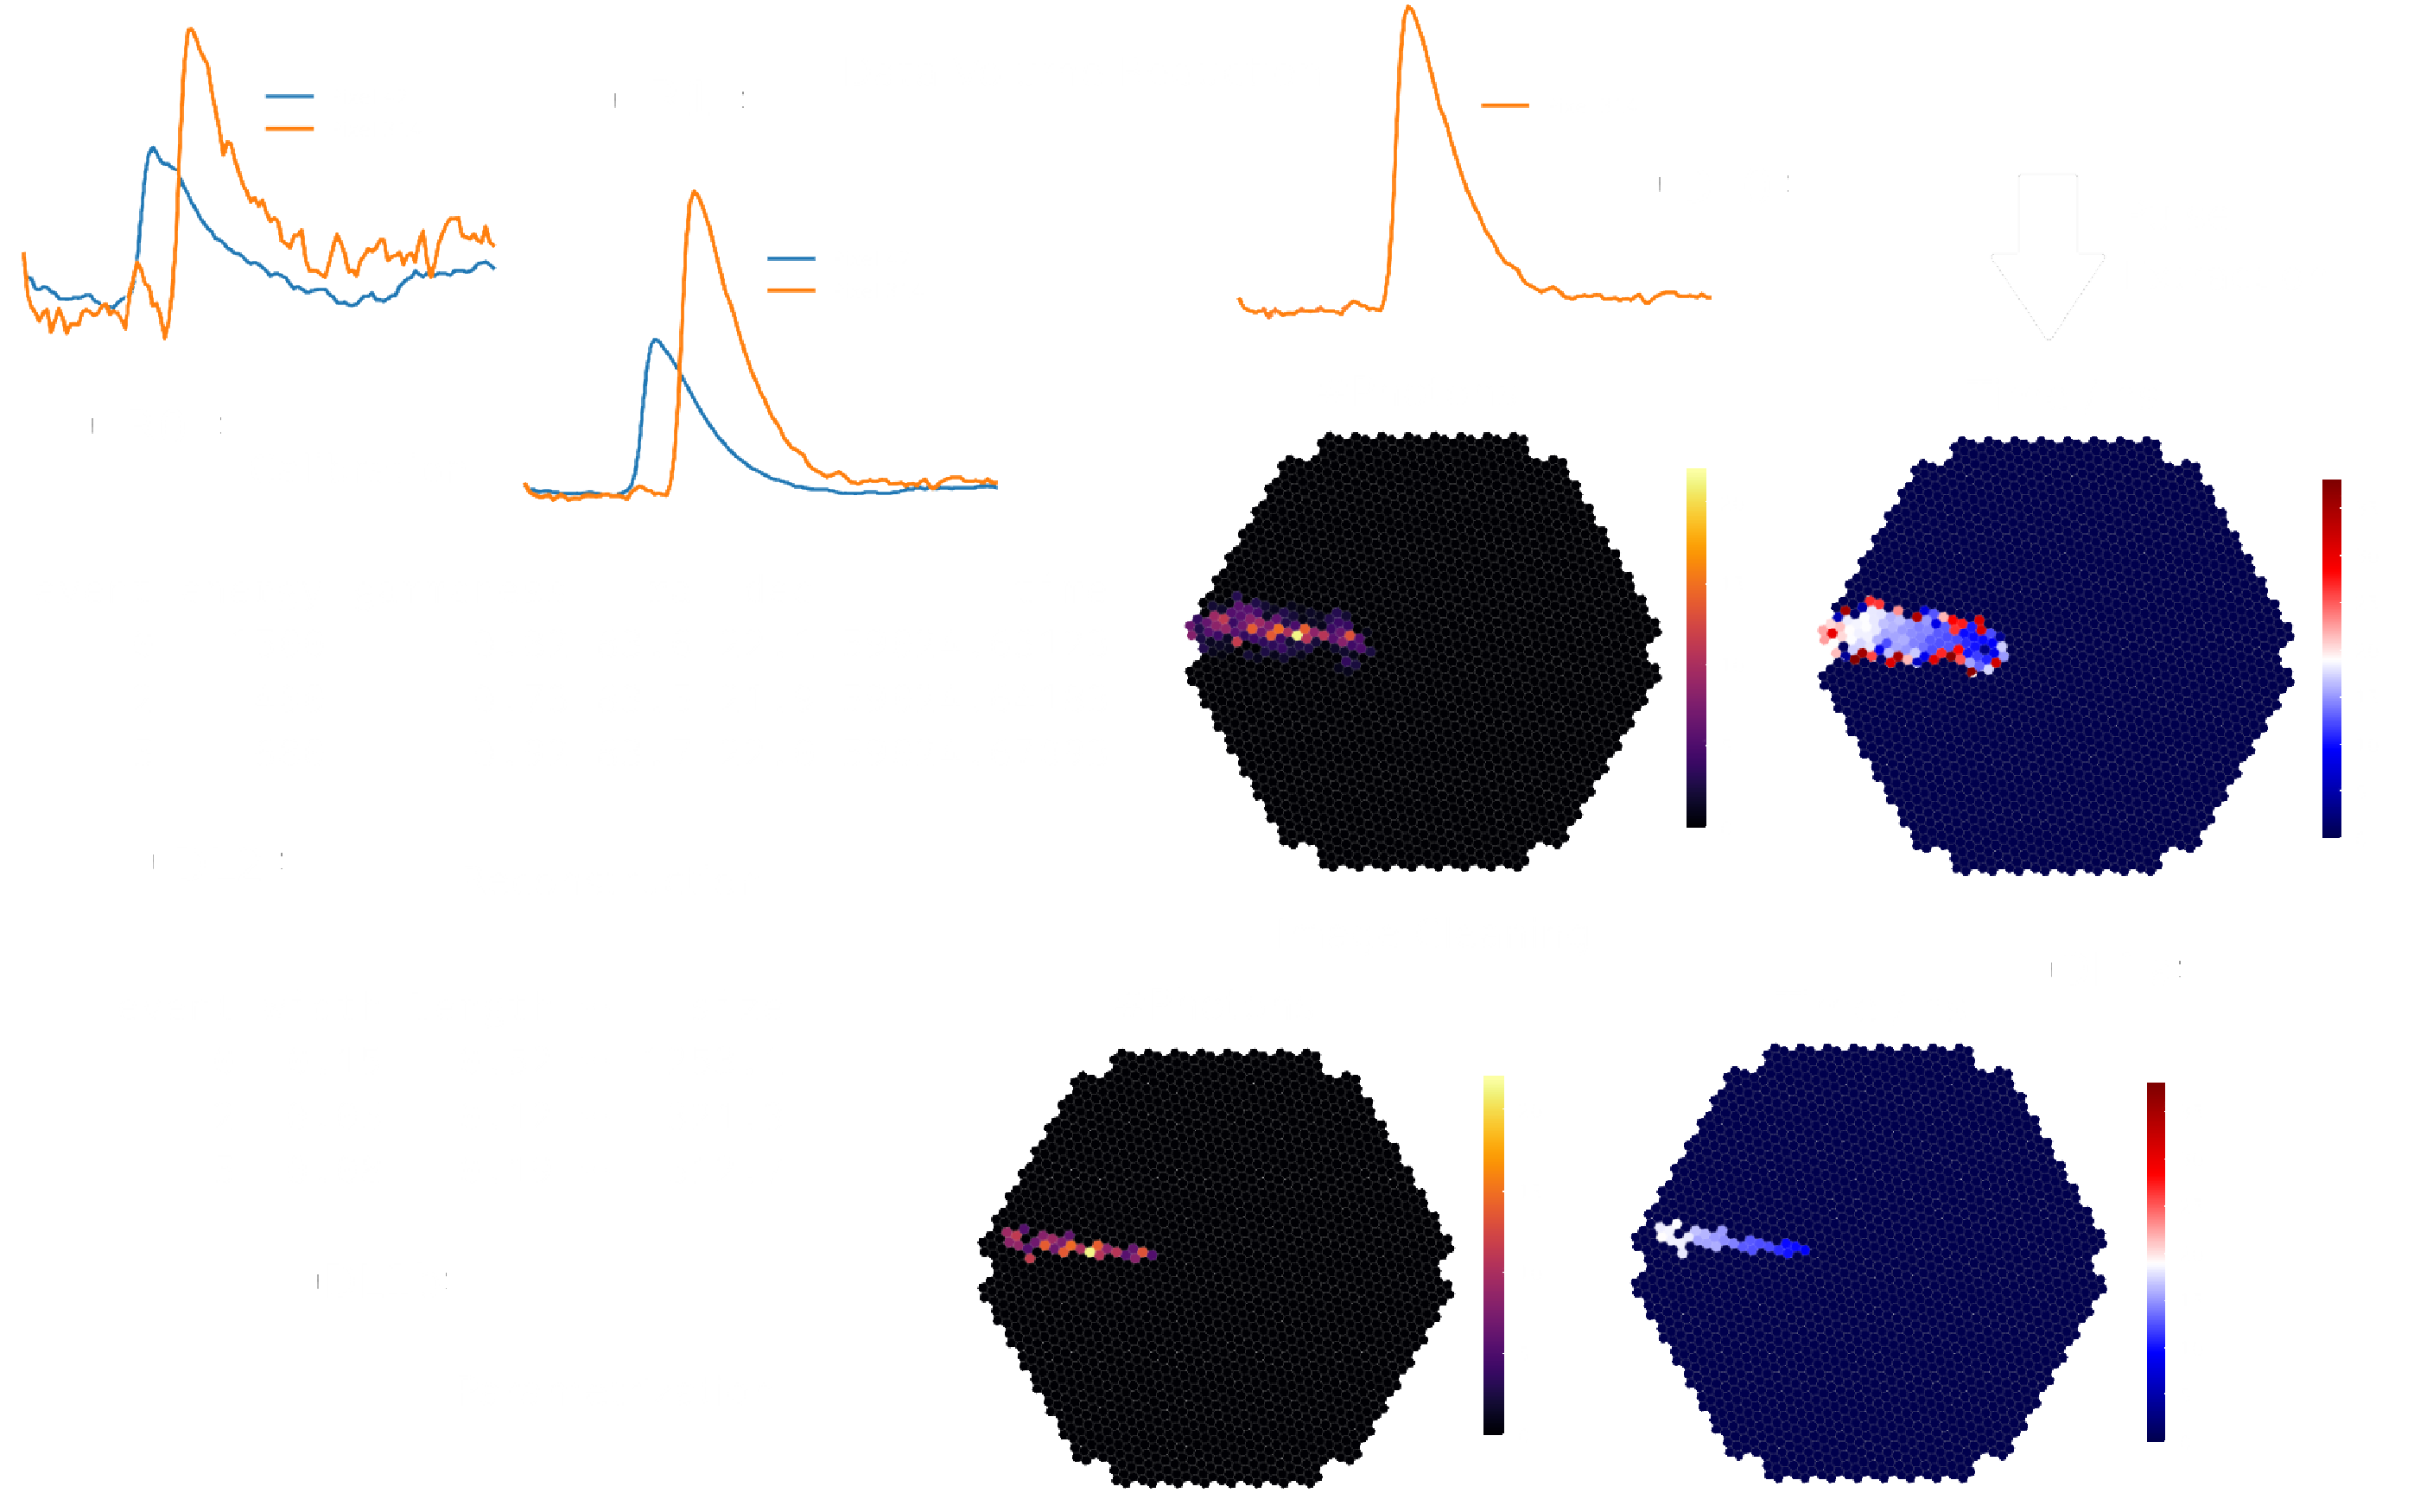
\includegraphics[height=0.9\textheight]{graphics/ctapipe_light.pdf}
    \vspace{-0.25cm}
    \footnote{\textcolor{white!85!black}{Adapted from J.~Hackfeld and M.~Linhoff}}
    }
    {% use light theme
    \centering
    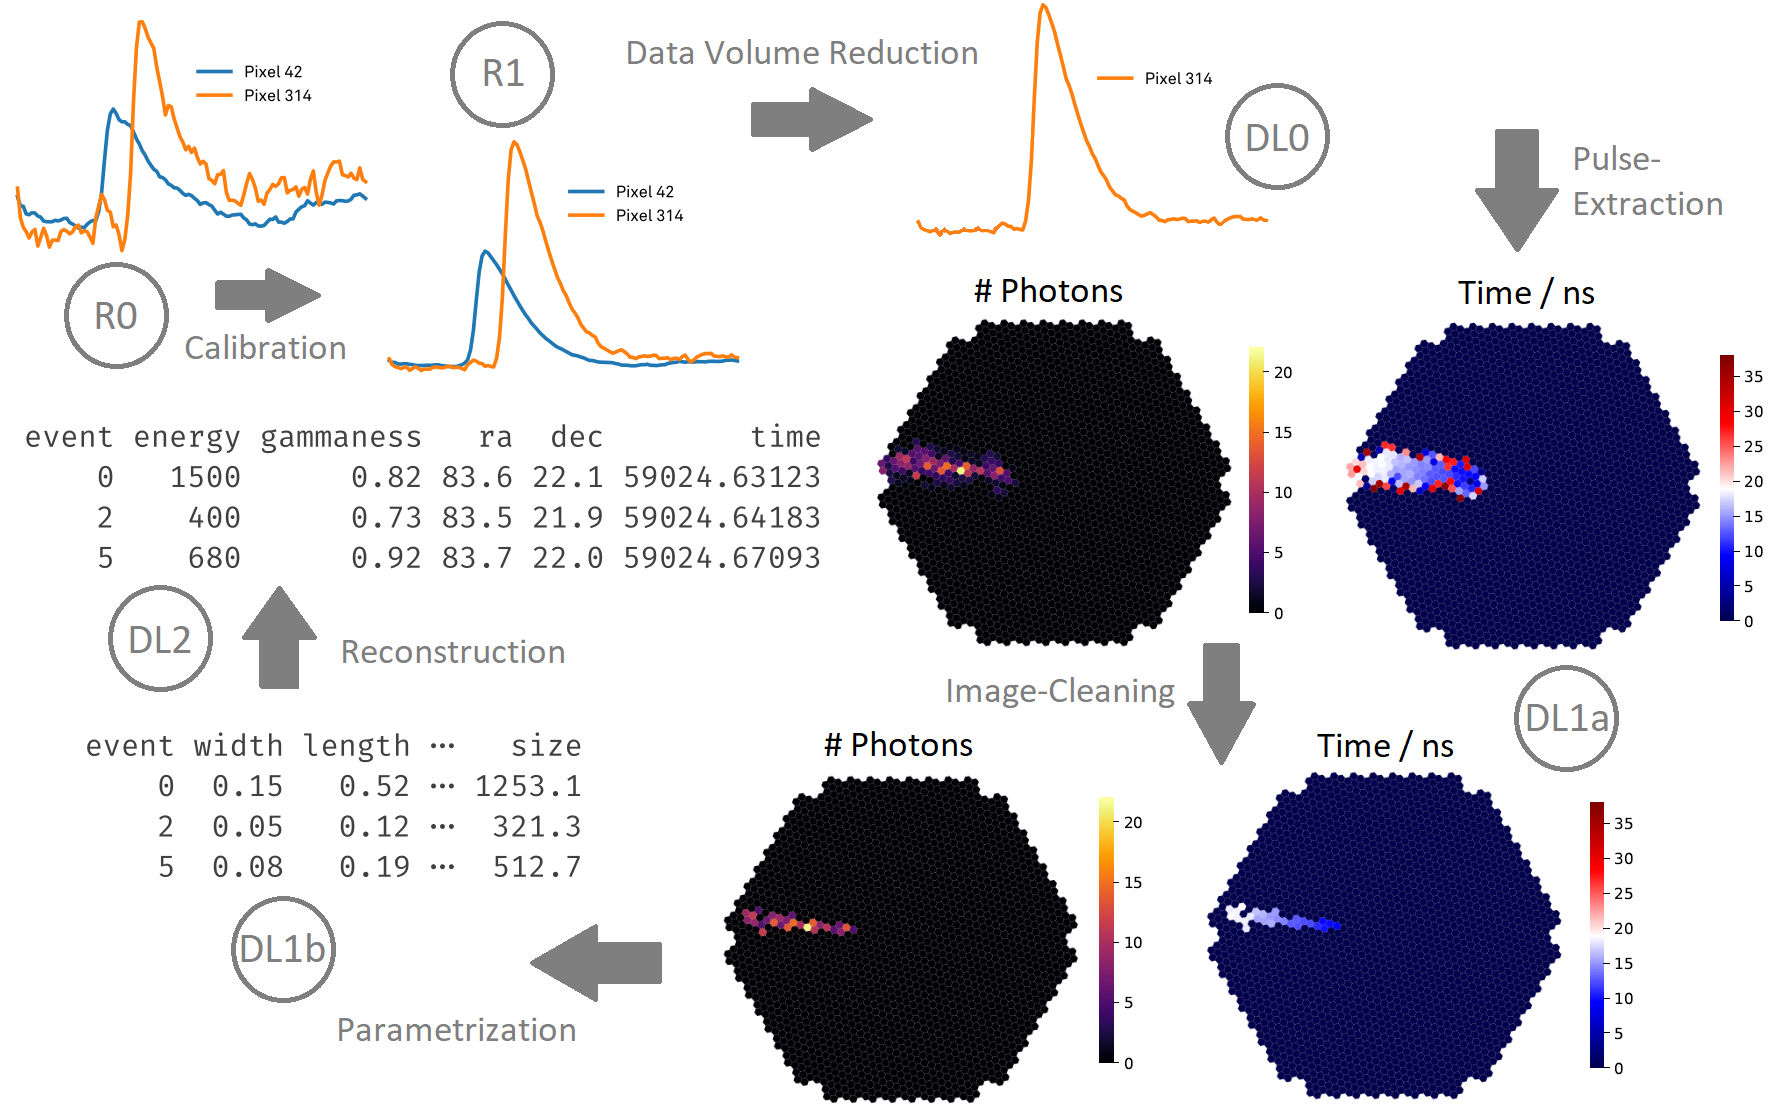
\includegraphics[height=0.9\textheight]{graphics/ctapipe.png}
    \vspace{-0.25cm}
    \footnote{\textcolor{darkgray!85!black}{Adapted from J.~Hackfeld and M.~Linhoff}}
    }
\end{frame}

\subsection{Cleaning Algorithms}%
\label{sub:Cleaning_algorithms}

\ifthenelse{\equal{\theme}{\string 1}}
    {% use dark theme
    \begin{frame}[t]{Cleaning Algorithms}
    \raisebox{10ex}{
    \begin{overlayarea}{0.36\textwidth}{3.5cm}
      \only<1>{
      \begin{itemize}
        \setlength\itemsep{1em}
        \item \code{white}{TailcutsImageCleaner}
        \item \code{white}{MARSImageCleaner}
        \item \code{white}{FACTImageCleaner}
        \item \code{white}{TimeConstrainedImageCleaner}
      \end{itemize}
      }
      \only<2>{
      \begin{itemize}
        \setlength\itemsep{1em}
        \item \code{white}{TailcutsImageCleaner}
        \item \code{white!50!black}{MARSImageCleaner}
        \item \code{white!50!black}{FACTImageCleaner}
        \item \code{white!50!black}{TimeConstrainedImageCleaner}
      \end{itemize}
      }
      \only<3>{
        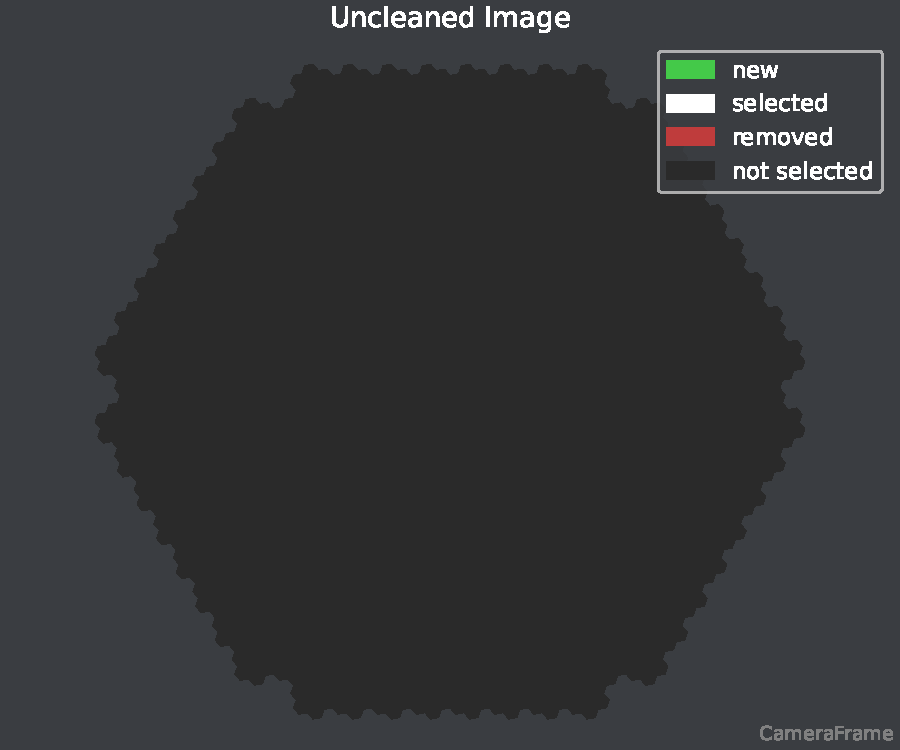
\includegraphics[width=\textwidth]{plots/cleaner_steps/dark/null_image.pdf}
      }
      \only<4>{
        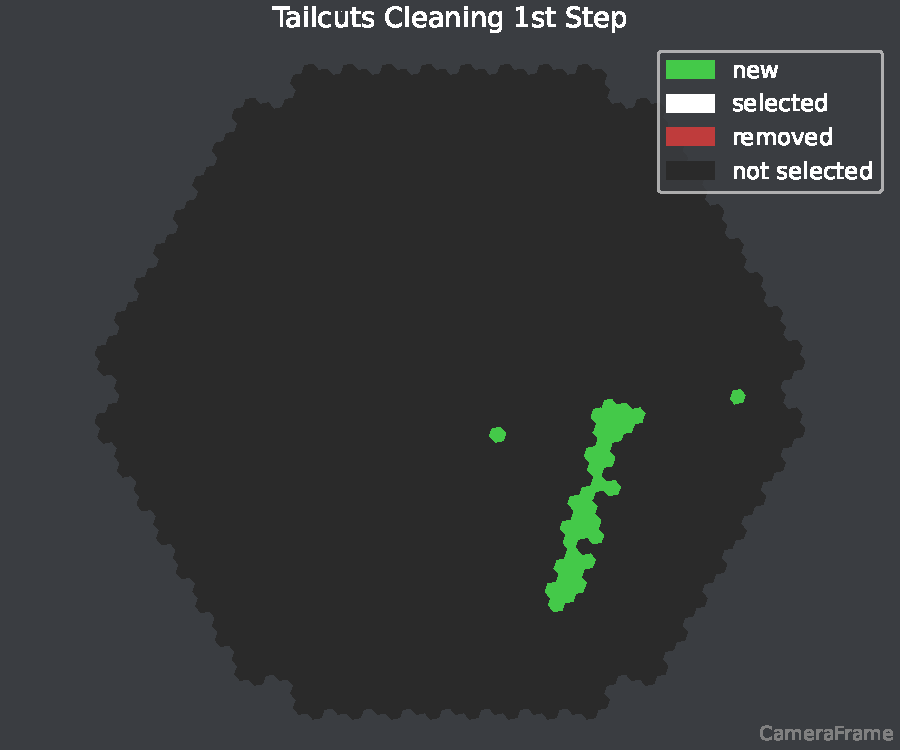
\includegraphics[width=\textwidth]{plots/cleaner_steps/dark/tail_1.pdf}
      }
      \only<5>{
        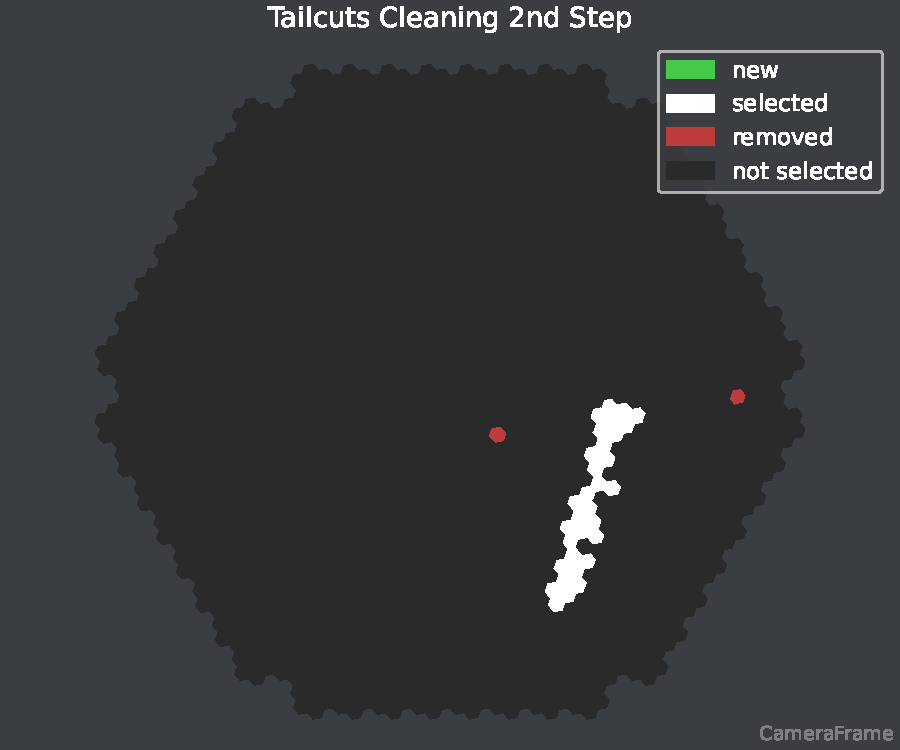
\includegraphics[width=\textwidth]{plots/cleaner_steps/dark/tail_2.pdf}
      }
      \only<6>{
      \begin{itemize}
        \setlength\itemsep{1em}
        \item \code{white!50!black}{TailcutsImageCleaner}
        \item \code{white}{MARSImageCleaner}
        \item \code{white!50!black}{FACTImageCleaner}
        \item \code{white!50!black}{TimeConstrainedImageCleaner}
      \end{itemize}
      }
      \only<7>{
        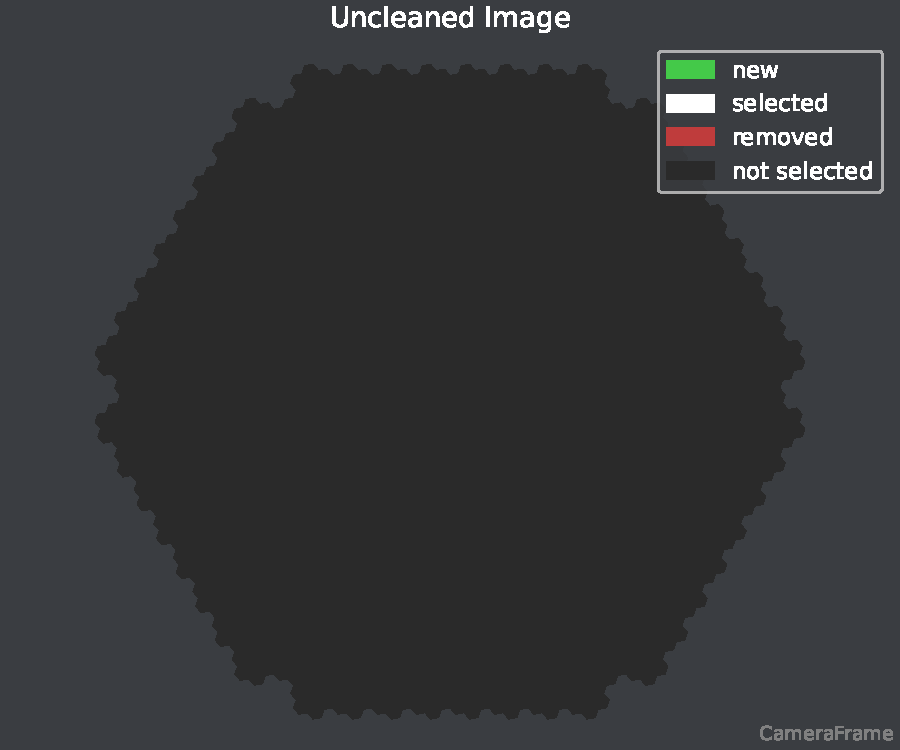
\includegraphics[width=\textwidth]{plots/cleaner_steps/dark/null_image.pdf}
      }
      \only<8>{
        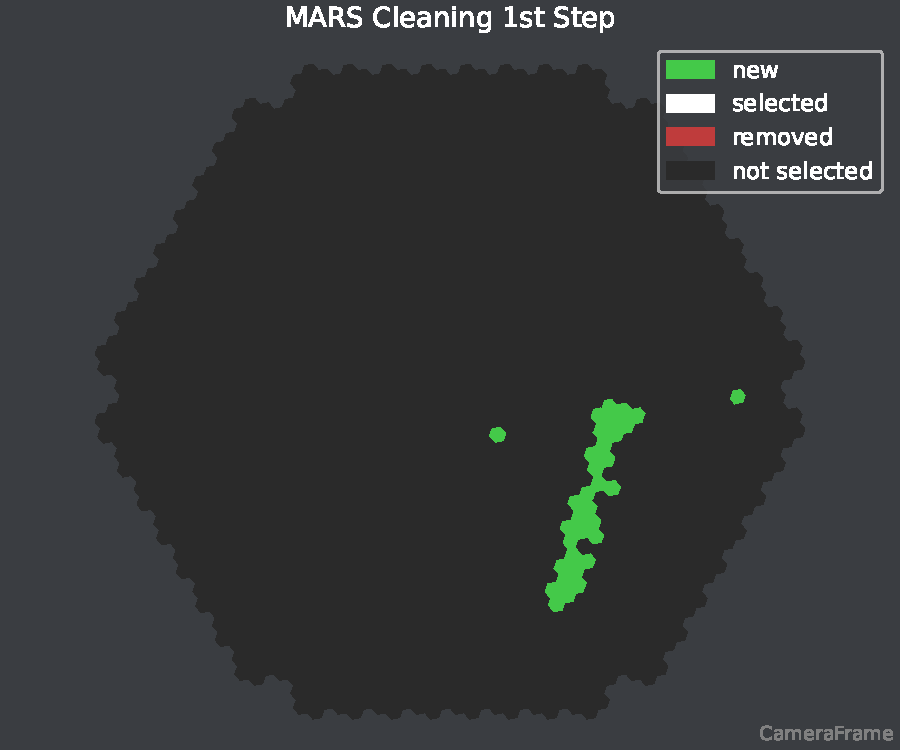
\includegraphics[width=\textwidth]{plots/cleaner_steps/dark/mars_1.pdf}
      }
      \only<9>{
        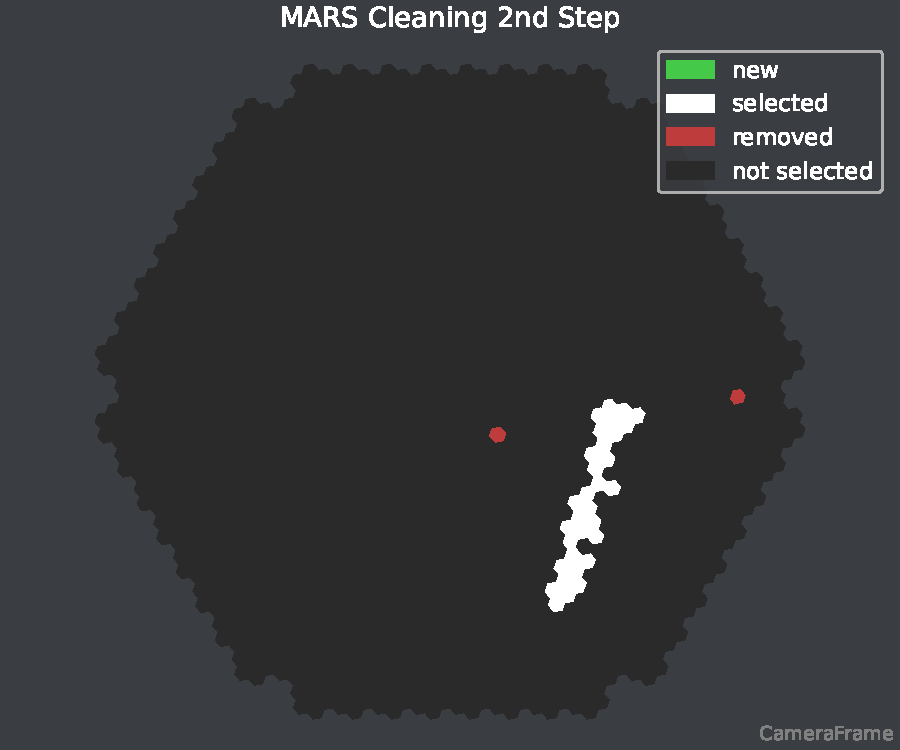
\includegraphics[width=\textwidth]{plots/cleaner_steps/dark/mars_2.pdf}
      }
      \only<10>{
        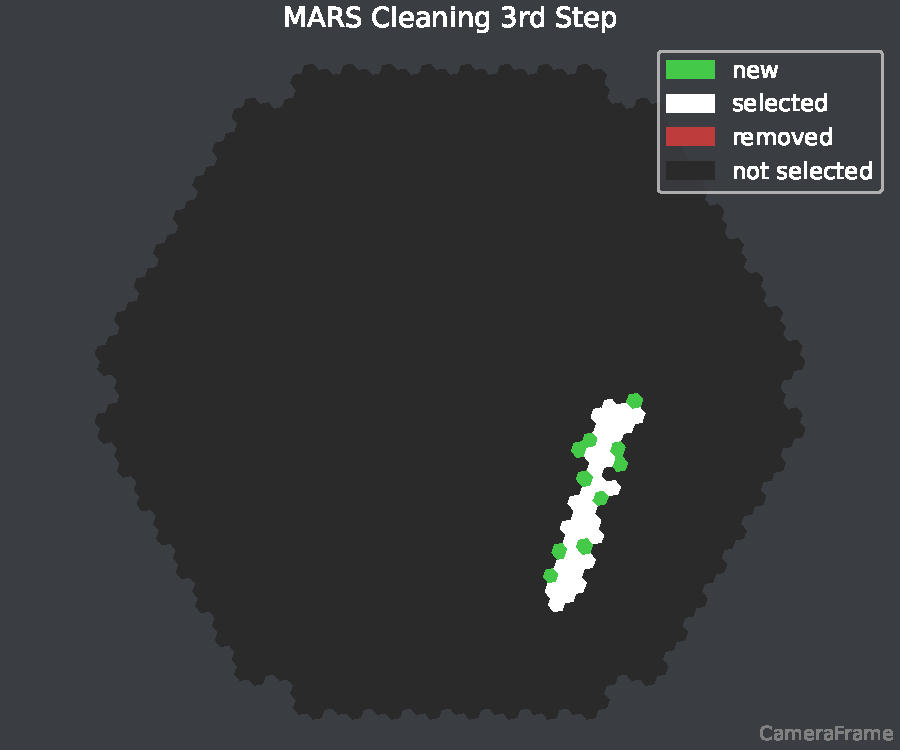
\includegraphics[width=\textwidth]{plots/cleaner_steps/dark/mars_3.pdf}
      }
      \only<11>{
      \begin{itemize}
        \setlength\itemsep{1em}
        \item \code{white!50!black}{TailcutsImageCleaner}
        \item \code{white!50!black}{MARSImageCleaner}
        \item \code{white}{FACTImageCleaner}
        \item \code{white!50!black}{TimeConstrainedImageCleaner}
      \end{itemize}
      }
      \only<12>{
        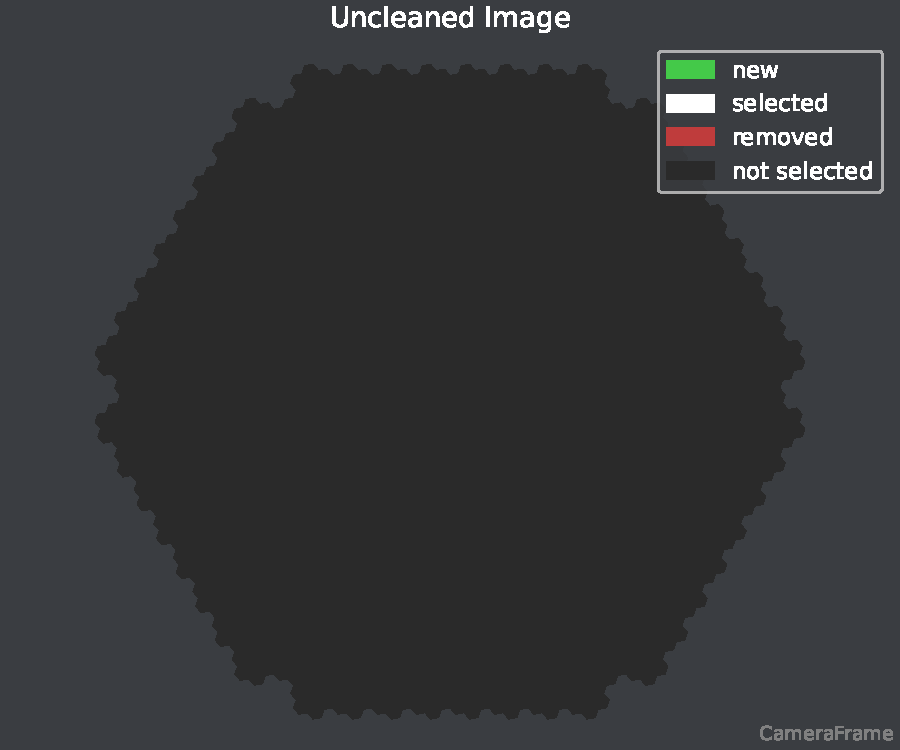
\includegraphics[width=\textwidth]{plots/cleaner_steps/dark/null_image.pdf}
      }
      \only<13>{
        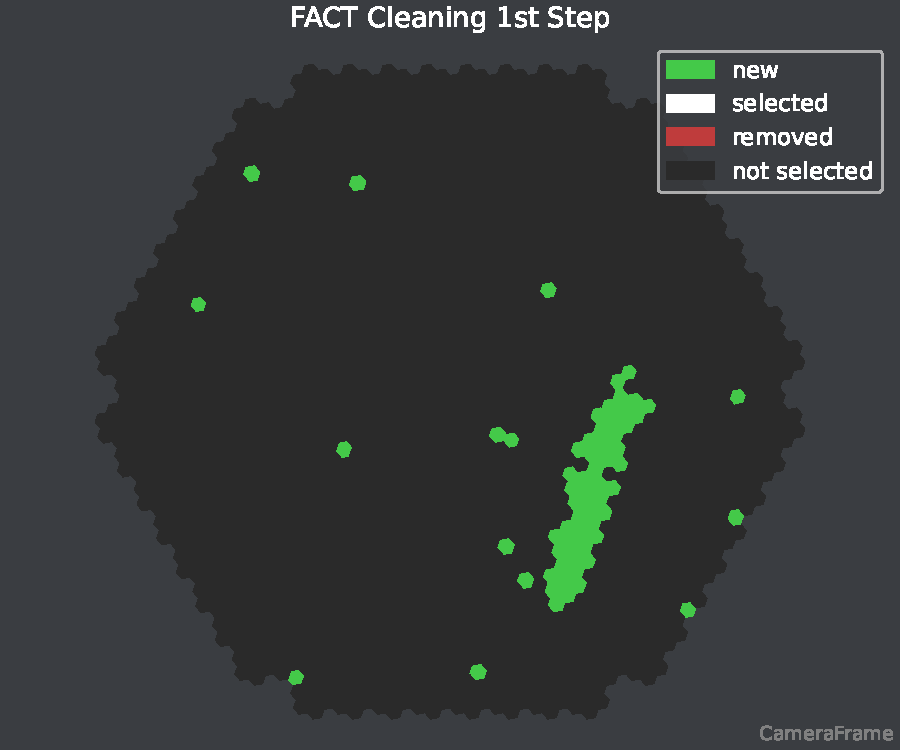
\includegraphics[width=\textwidth]{plots/cleaner_steps/dark/fact_1.pdf}
      }
      \only<14>{
        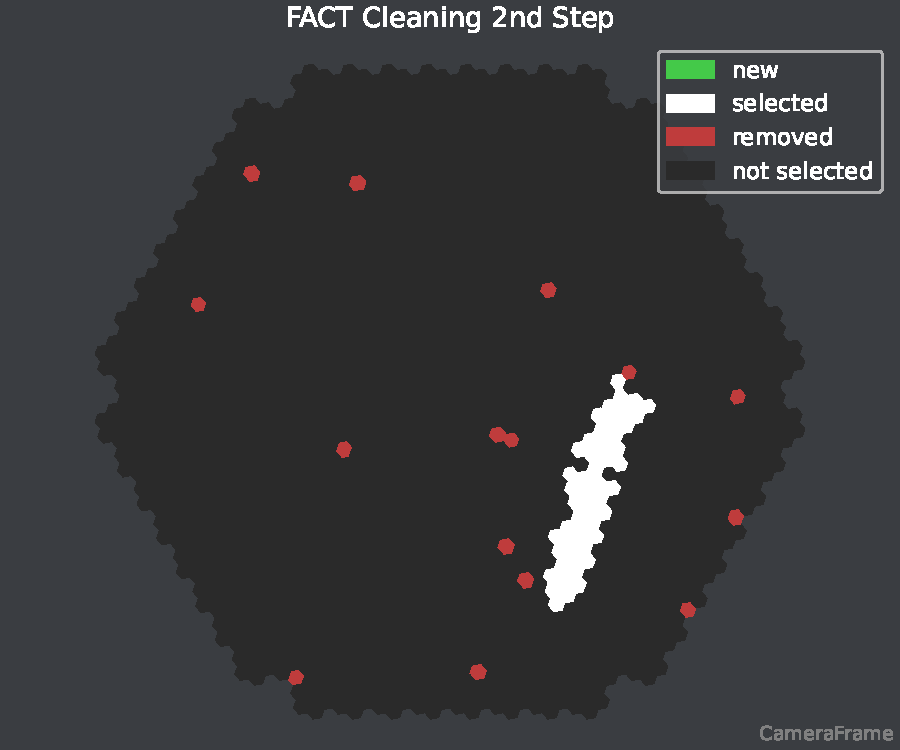
\includegraphics[width=\textwidth]{plots/cleaner_steps/dark/fact_2.pdf}
      }
      \only<15>{
        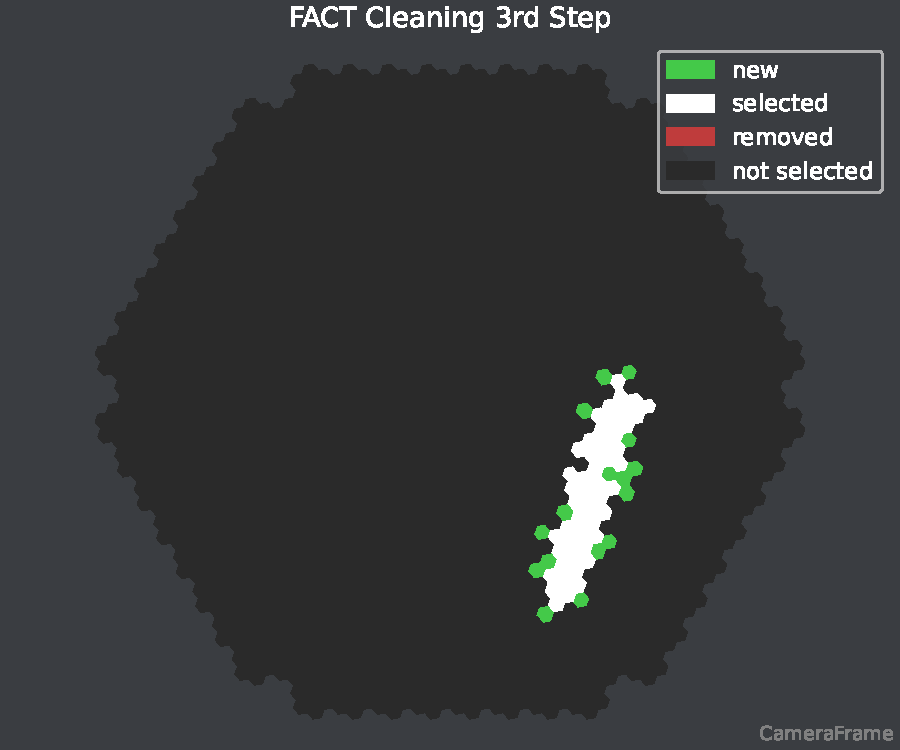
\includegraphics[width=\textwidth]{plots/cleaner_steps/dark/fact_3.pdf}
      }
      \only<16>{
        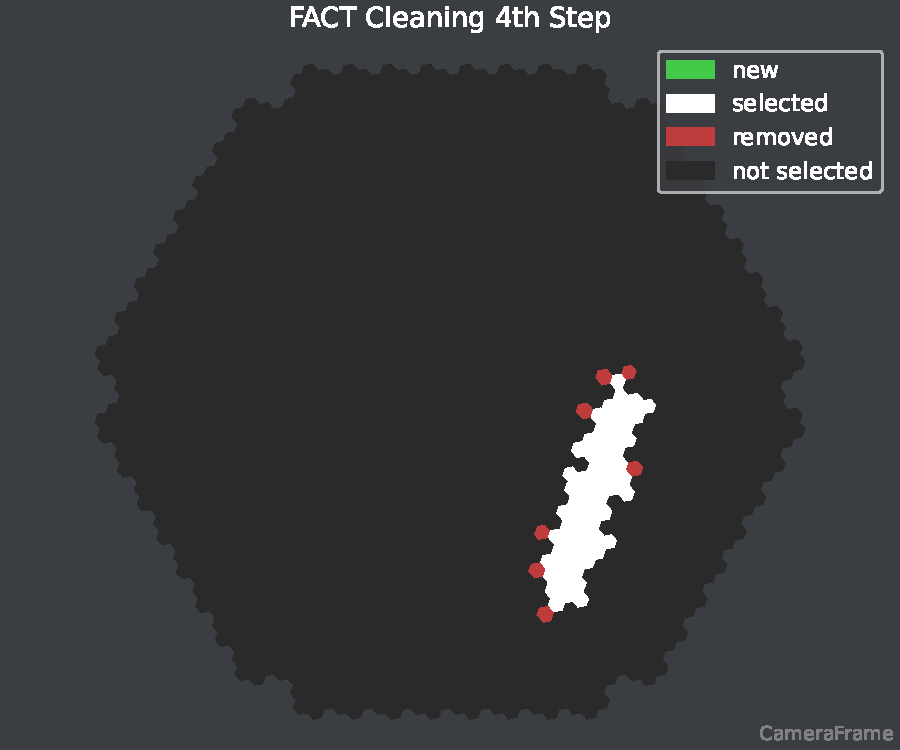
\includegraphics[width=\textwidth]{plots/cleaner_steps/dark/fact_4.pdf}
      }
      \only<17>{
        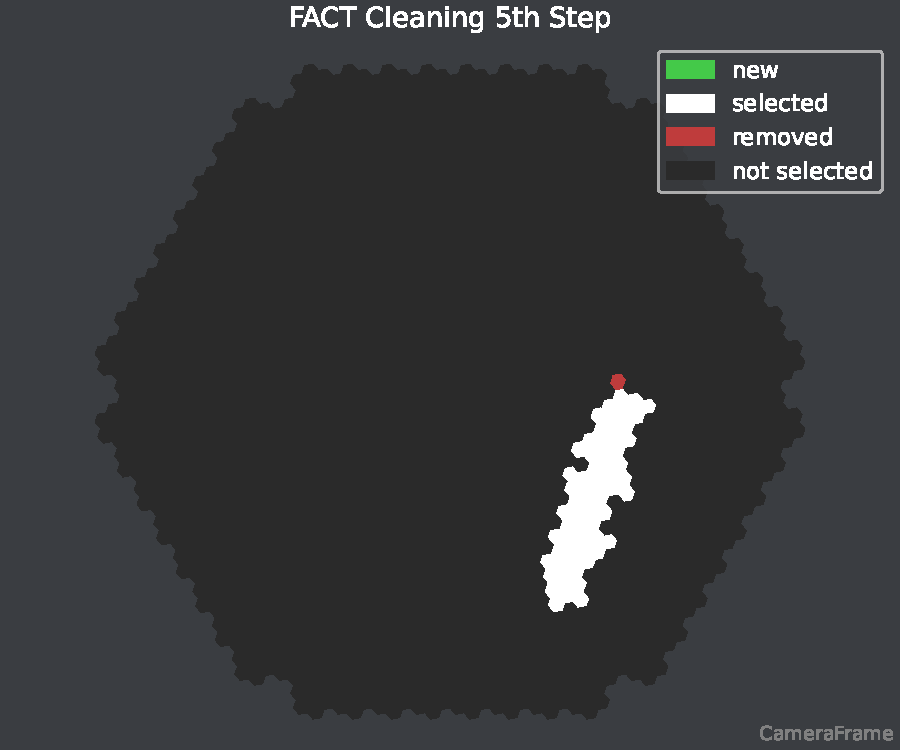
\includegraphics[width=\textwidth]{plots/cleaner_steps/dark/fact_5.pdf}
      }
      \only<18>{
        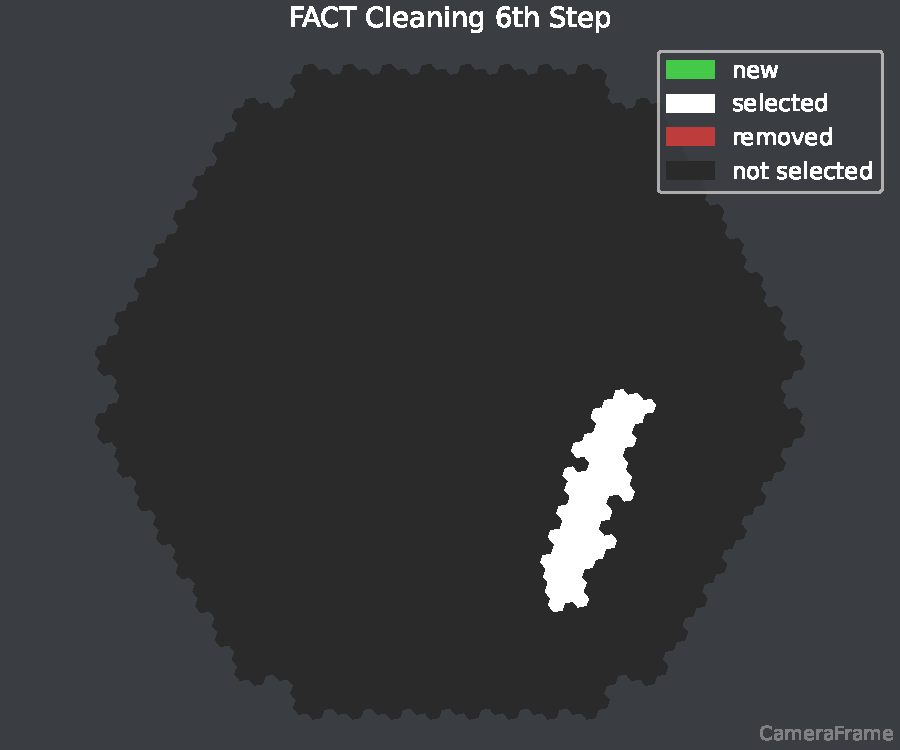
\includegraphics[width=\textwidth]{plots/cleaner_steps/dark/fact_6.pdf}
      }
      \only<19>{
      \begin{itemize}
        \setlength\itemsep{1em}
        \item \code{white!50!black}{TailcutsImageCleaner}
        \item \code{white!50!black}{MARSImageCleaner}
        \item \code{white!50!black}{FACTImageCleaner}
        \item \code{white}{TimeConstrainedImageCleaner}
      \end{itemize}
      }
      \only<20>{
        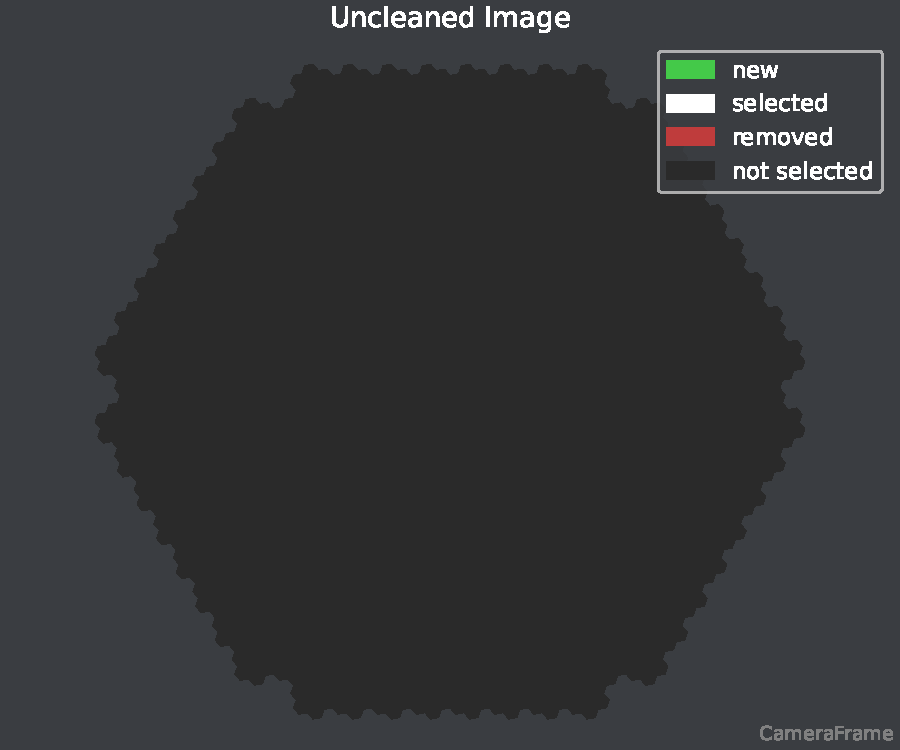
\includegraphics[width=\textwidth]{plots/cleaner_steps/dark/null_image.pdf}
      }
      \only<21>{
        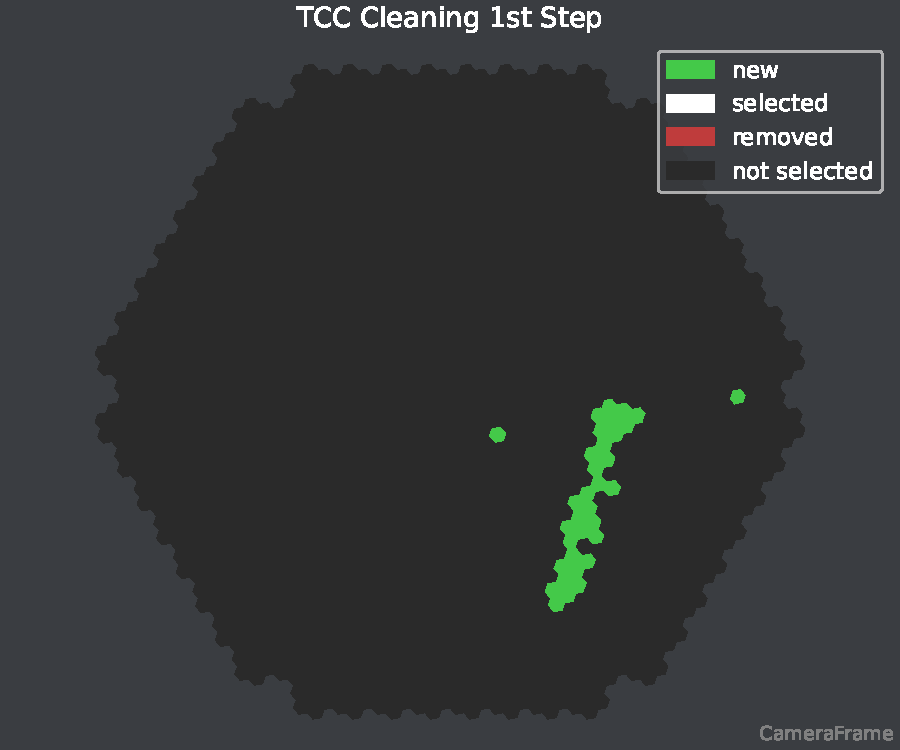
\includegraphics[width=\textwidth]{plots/cleaner_steps/dark/tcc_1.pdf}
      }
      \only<22>{
        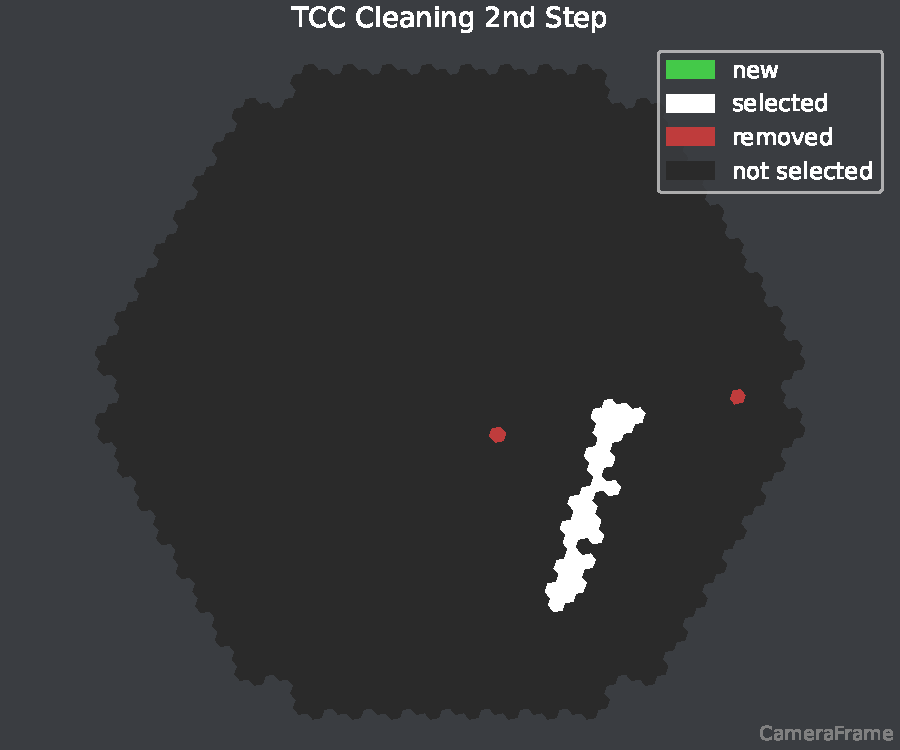
\includegraphics[width=\textwidth]{plots/cleaner_steps/dark/tcc_2.pdf}
      }
      \only<23>{
        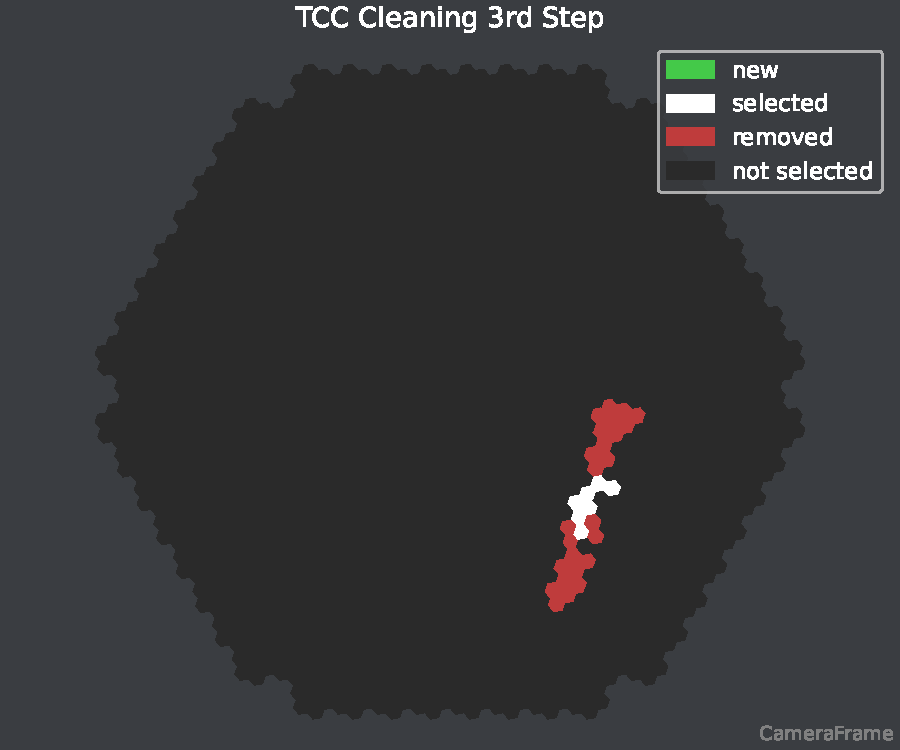
\includegraphics[width=\textwidth]{plots/cleaner_steps/dark/tcc_3.pdf}
      }
      \only<24>{
        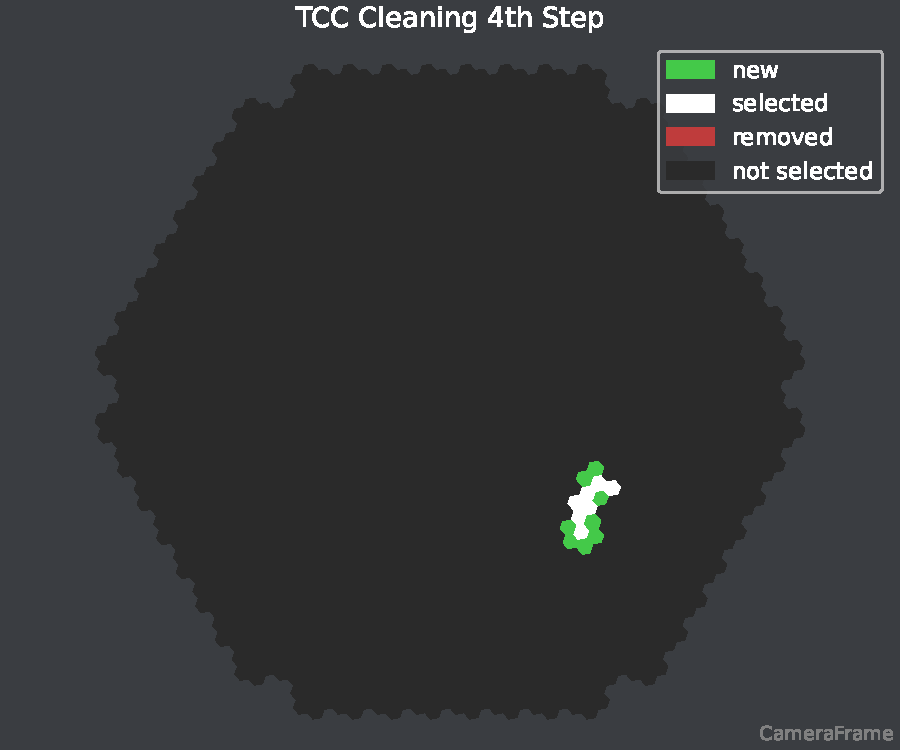
\includegraphics[width=\textwidth]{plots/cleaner_steps/dark/tcc_4.pdf}
      }
      \only<25>{
        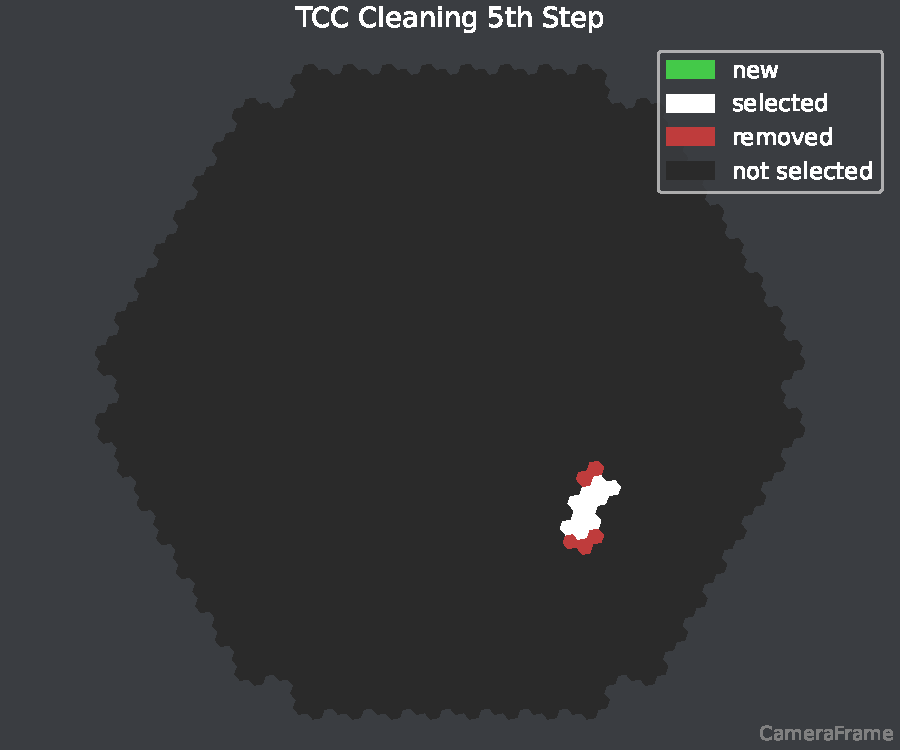
\includegraphics[width=\textwidth]{plots/cleaner_steps/dark/tcc_5.pdf}
      }
    \end{overlayarea}
    }
    \raisebox{10ex}{
    \begin{overlayarea}{0.58\textwidth}{3.5cm}
      \only<1>{
        \centering
        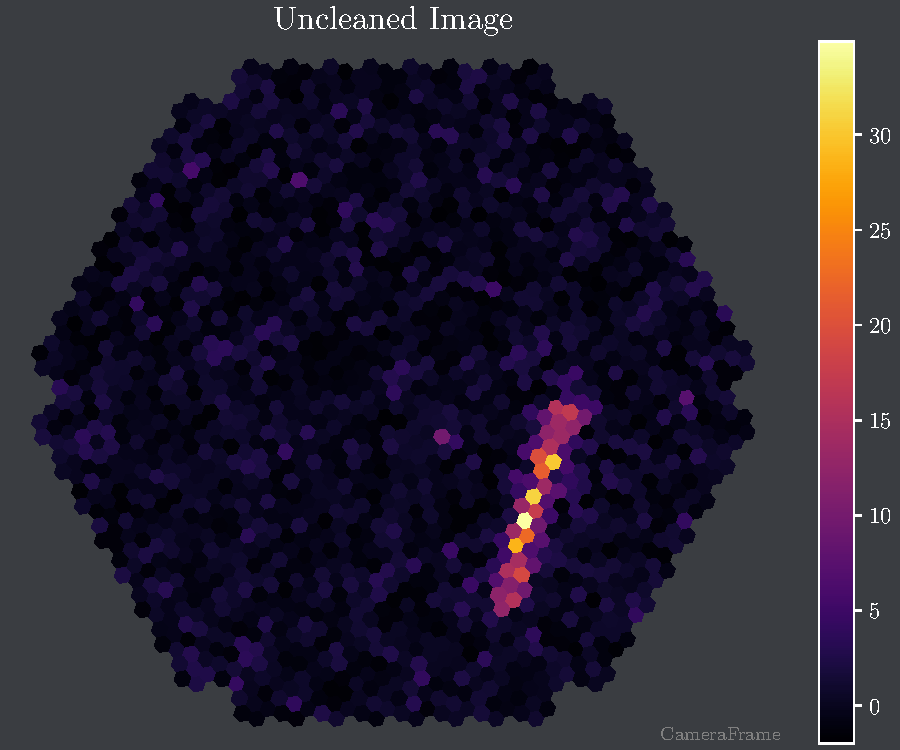
\includegraphics[width=0.65\textwidth]{plots/cleaner_steps/dark/uncleaned_image.pdf}
      }
      \only<2>{
      \begin{enumerate}%TailcutsImageCleaner
        \item Select pixels that pass the \code{white!70!black}{core threshold} (\(Q_c = \SI{7}{\pe}\))
        \item Add pixels that pass the \code{white!70!black}{boundary threshold} (\(Q_b = \SI{5}{\pe}\))
      \end{enumerate}
      }
      \only<3>{
      \begin{enumerate}%TailcutsImageCleaner
        \item \textcolor{white!50!black}{Select pixels that pass the \code{white!35!black}{core threshold} (\(Q_c = \SI{7}{\pe}\))}
        \item \textcolor{white!50!black}{Add pixels that pass the \code{white!35!black}{boundary threshold} (\(Q_b = \SI{5}{\pe}\))}
      \end{enumerate}
      }
      \only<4>{
      \begin{enumerate}%TailcutsImageCleaner
        \item Select pixels that pass the \code{white!70!black}{core threshold} (\(Q_c = \SI{7}{\pe}\))
        \item \textcolor{white!50!black}{Add pixels that pass the \code{white!35!black}{boundary threshold} (\(Q_b = \SI{5}{\pe}\))}
      \end{enumerate}
      }
      \only<5>{
      \begin{enumerate}%TailcutsImageCleaner
        \item \textcolor{white!50!black}{Select pixels that pass the \code{white!35!black}{core threshold} (\(Q_c = \SI{7}{\pe}\))}
        \item Add pixels that pass the \code{white!70!black}{boundary threshold} (\(Q_b = \SI{5}{\pe}\))
      \end{enumerate}
      }

      \only<6>{
      \begin{enumerate}%MARSImageCleaner
        \item Select pixels that pass the \code{white!70!black}{core} and \code{white!70!black}{boundary threshold}, analogous to \code{white!70!black}{TailcutsImageCleaner}
        \item Add pixels that are a neighbor of a neighbor of a core pixel, if they are above the \code{white!70!black}{boundary threshold}
      \end{enumerate}
      }
      \only<7>{
      \begin{enumerate}%MARSImageCleaner
        \item \textcolor{white!50!black}{Select pixels that pass the \code{white!35!black}{core} and \code{white!35!black}{boundary threshold}, analogous to \code{white!35!black}{TailcutsImageCleaner}}
        \item \textcolor{white!50!black}{Add pixels that are a neighbor of a neighbor of a core pixel, if they are above the \code{white!35!black}{boundary threshold}}
      \end{enumerate}
      }
      \only<8-9>{
      \begin{enumerate}%MARSImageCleaner
        \item Select pixels that pass the \code{white!70!black}{core} and \code{white!70!black}{boundary threshold}, analogous to \code{white!70!black}{TailcutsImageCleaner}
        \item \textcolor{white!50!black}{Add pixels that are a neighbor of a neighbor of a core pixel, if they are above the \code{white!35!black}{boundary threshold}}
      \end{enumerate}
      }
      \only<10>{
      \begin{enumerate}%MARSImageCleaner
        \item \textcolor{white!50!black}{Select pixels that pass the \code{white!35!black}{core} and \code{white!35!black}{boundary threshold}, analogous to \code{white!35!black}{TailcutsImageCleaner}}
        \item Add pixels that are a neighbor of a neighbor of a core pixel, if they are above the \code{white!70!black}{boundary threshold}
      \end{enumerate}
      }
      \only<11>{
      \begin{enumerate}%FACTImageCleaner
        \item Find all pixels that contain more photons than the \code{white!70!black}{core threshold} (\(Q_c = \SI{4}{\pe}\))
        \item Remove pixels with less than \(N\) neighbors (this talk: \(N=2\))
        \item Add remaining neighbors that are above the \code{white!70!black}{boundary threshold} (\(Q_b = \SI{2}{\pe}\))
        \item Remove pixels that have less than \(N\) neighbors, that arrive within a given timeframe (\(t = \SI{5}{\nano\second}\))
        \item Remove pixels that have less than \(N\) neighbors
        \item Remove pixels that have less than \(N\) neighbors, arriving within a given timeframe (same as in step 4)
      \end{enumerate}
      }
      \only<12>{
      \begin{enumerate}%FACTImageCleaner
        \item \textcolor{white!50!black}{Find all pixels that contain more photons than the \code{white!35!black}{core threshold} (\(Q_c = \SI{4}{\pe}\))}
        \item \textcolor{white!50!black}{Remove pixels with less than \(N\) neighbors (this talk: \(N=2\))}
        \item \textcolor{white!50!black}{Add remaining neighbors that are above the \code{white!35!black}{boundary threshold} (\(Q_b = \SI{2}{\pe}\))}
        \item \textcolor{white!50!black}{Remove pixels that have less than \(N\) neighbors, that arrive within a given timeframe (\(t = \SI{5}{\nano\second}\))}
        \item \textcolor{white!50!black}{Remove pixels that have less than \(N\) neighbors}
        \item \textcolor{white!50!black}{Remove pixels that have less than \(N\) neighbors, arriving within a given timeframe (same as in step 4)}
      \end{enumerate}
      }
      \only<13>{
      \begin{enumerate}%FACTImageCleaner
        \item Find all pixels that contain more photons than the \code{white!70!black}{core threshold} (\(Q_c = \SI{4}{\pe}\))
        \item \textcolor{white!50!black}{Remove pixels with less than \(N\) neighbors (this talk: \(N=2\))}
        \item \textcolor{white!50!black}{Add remaining neighbors that are above the \code{white!35!black}{boundary threshold} (\(Q_b = \SI{2}{\pe}\))}
        \item \textcolor{white!50!black}{Remove pixels that have less than \(N\) neighbors, that arrive within a given timeframe (\(t = \SI{5}{\nano\second}\))}
        \item \textcolor{white!50!black}{Remove pixels that have less than \(N\) neighbors}
        \item \textcolor{white!50!black}{Remove pixels that have less than \(N\) neighbors, arriving within a given timeframe (same as in step 4)}
      \end{enumerate}
      }
      \only<14>{
      \begin{enumerate}%FACTImageCleaner
        \item \textcolor{white!50!black}{Find all pixels that contain more photons than the \code{white!35!black}{core threshold} (\(Q_c = \SI{4}{\pe}\))}
        \item Remove pixels with less than \(N\) neighbors (this talk: \(N=2\))
        \item \textcolor{white!50!black}{Add remaining neighbors that are above the \code{white!35!black}{boundary threshold} (\(Q_b = \SI{2}{\pe}\))}
        \item \textcolor{white!50!black}{Remove pixels that have less than \(N\) neighbors, that arrive within a given timeframe (\(t = \SI{5}{\nano\second}\))}
        \item \textcolor{white!50!black}{Remove pixels that have less than \(N\) neighbors}
        \item \textcolor{white!50!black}{Remove pixels that have less than \(N\) neighbors, arriving within a given timeframe (same as in step 4)}
      \end{enumerate}
      }
      \only<15>{
      \begin{enumerate}%FACTImageCleaner
        \item \textcolor{white!50!black}{Find all pixels that contain more photons than the \code{white!35!black}{core threshold} (\(Q_c = \SI{4}{\pe}\))}
        \item \textcolor{white!50!black}{Remove pixels with less than \(N\) neighbors (this talk: \(N=2\))}
        \item Add remaining neighbors that are above the \code{white!70!black}{boundary threshold} (\(Q_b = \SI{2}{\pe}\))
        \item \textcolor{white!50!black}{Remove pixels that have less than \(N\) neighbors, that arrive within a given timeframe (\(t = \SI{5}{\nano\second}\))}
        \item \textcolor{white!50!black}{Remove pixels that have less than \(N\) neighbors}
        \item \textcolor{white!50!black}{Remove pixels that have less than \(N\) neighbors, arriving within a given timeframe (same as in step 4)}
      \end{enumerate}
      }
      \only<16>{
      \begin{enumerate}%FACTImageCleaner
        \item \textcolor{white!50!black}{Find all pixels that contain more photons than the \code{white!35!black}{core threshold} (\(Q_c = \SI{4}{\pe}\))}
        \item \textcolor{white!50!black}{Remove pixels with less than \(N\) neighbors (this talk: \(N=2\))}
        \item \textcolor{white!50!black}{Add remaining neighbors that are above the \code{white!35!black}{boundary threshold} (\(Q_b = \SI{2}{\pe}\))}
        \item Remove pixels that have less than \(N\) neighbors, that arrive within a given timeframe (\(t = \SI{5}{\nano\second}\))
        \item \textcolor{white!50!black}{Remove pixels that have less than \(N\) neighbors}
        \item \textcolor{white!50!black}{Remove pixels that have less than \(N\) neighbors, arriving within a given timeframe (same as in step 4)}
      \end{enumerate}
      }
      \only<17>{
      \begin{enumerate}%FACTImageCleaner
        \item \textcolor{white!50!black}{Find all pixels that contain more photons than the \code{white!35!black}{core threshold} (\(Q_c = \SI{4}{\pe}\))}
        \item \textcolor{white!50!black}{Remove pixels with less than \(N\) neighbors (this talk: \(N=2\))}
        \item \textcolor{white!50!black}{Add remaining neighbors that are above the \code{white!35!black}{boundary threshold} (\(Q_b = \SI{2}{\pe}\))}
        \item \textcolor{white!50!black}{Remove pixels that have less than \(N\) neighbors, that arrive within a given timeframe (\(t = \SI{5}{\nano\second}\))}
        \item Remove pixels that have less than \(N\) neighbors
        \item \textcolor{white!50!black}{Remove pixels that have less than \(N\) neighbors, arriving within a given timeframe (same as in step 4)}
      \end{enumerate}
      }
      \only<18>{
      \begin{enumerate}%FACTImageCleaner
        \item \textcolor{white!50!black}{Find all pixels that contain more photons than the \code{white!35!black}{core threshold} (\(Q_c = \SI{4}{\pe}\))}
        \item \textcolor{white!50!black}{Remove pixels with less than \(N\) neighbors (this talk: \(N=2\))}
        \item \textcolor{white!50!black}{Add remaining neighbors that are above the \code{white!35!black}{boundary threshold} (\(Q_b = \SI{2}{\pe}\))}
        \item \textcolor{white!50!black}{Remove pixels that have less than \(N\) neighbors, that arrive within a given timeframe (\(t = \SI{5}{\nano\second}\))}
        \item \textcolor{white!50!black}{Remove pixels that have less than \(N\) neighbors}
        \item Remove pixels that have less than \(N\) neighbors, arriving within the given timeframe (same as in step 4)
      \end{enumerate}
      }
      \only<19>{
      \begin{enumerate}%TimeConstrainedImageCleaner
        \item Find all core pixels above the \code{white!70!black}{core threshold} (\(Q_c = \SI{7}{\pe}\))
        \item Remove pixels with less than \(N\) neighbors (this talk: \(N=1\))
        \item Keep all pixels that arrive within a time limit of the average arrival time (\(t_c = \SI{4.5}{\nano\second}\))
        \item Find all neighboring pixels above the \code{white!70!black}{boundary threshold} (\(Q_b = \SI{5}{\pe}\))
        \item Remove all pixels with less than \(N\) neighbors arriving within a given timeframe (\(t_b = \SI{1.5}{\nano\second}\))
      \end{enumerate}
      }
      \only<20>{
      \begin{enumerate}%TimeConstrainedImageCleaner
        \item \textcolor{white!50!black}{Find all core pixels above the \code{white!35!black}{core threshold} (\(Q_c = \SI{7}{\pe}\))}
        \item \textcolor{white!50!black}{Remove pixels with less than \(N\) neighbors (this talk: \(N=1\))}
        \item \textcolor{white!50!black}{Keep all pixels that arrive within a time limit of the average arrival time (\(t_c = \SI{4.5}{\nano\second}\))}
        \item \textcolor{white!50!black}{Find all neighboring pixels above the \code{white!35!black}{boundary threshold} (\(Q_b = \SI{5}{\pe}\))}
        \item \textcolor{white!50!black}{Remove all pixels with less than \(N\) neighbors arriving within a given timeframe (\(t_b = \SI{1.5}{\nano\second}\))}
      \end{enumerate}
      }
      \only<21>{
      \begin{enumerate}%TimeConstrainedImageCleaner
        \item Find all core pixels above the \code{white!70!black}{core threshold} (\(Q_c = \SI{7}{\pe}\))
        \item \textcolor{white!50!black}{Remove pixels with less than \(N\) neighbors (this talk: \(N=1\))}
        \item \textcolor{white!50!black}{Keep all pixels that arrive within a time limit of the average arrival time (\(t_c = \SI{4.5}{\nano\second}\))}
        \item \textcolor{white!50!black}{Find all neighboring pixels above the \code{white!35!black}{boundary threshold} (\(Q_b = \SI{5}{\pe}\))}
        \item \textcolor{white!50!black}{Remove all pixels with less than \(N\) neighbors arriving within a given timeframe (\(t_b = \SI{1.5}{\nano\second}\))}
      \end{enumerate}
      }
      \only<22>{
      \begin{enumerate}%TimeConstrainedImageCleaner
        \item \textcolor{white!50!black}{Find all core pixels above the \code{white!35!black}{core threshold} (\(Q_c = \SI{7}{\pe}\))}
        \item Remove pixels with less than \(N\) neighbors (this talk: \(N=1\))
        \item \textcolor{white!50!black}{Keep all pixels that arrive within a time limit of the average arrival time (\(t_c = \SI{4.5}{\nano\second}\))}
        \item \textcolor{white!50!black}{Find all neighboring pixels above the \code{white!35!black}{boundary threshold} (\(Q_b = \SI{5}{\pe}\))}
        \item \textcolor{white!50!black}{Remove all pixels with less than \(N\) neighbors arriving within a given timeframe (\(t_b = \SI{1.5}{\nano\second}\))}
      \end{enumerate}
      }
      \only<23>{
      \begin{enumerate}%TimeConstrainedImageCleaner
        \item \textcolor{white!50!black}{Find all core pixels above the \code{white!35!black}{core threshold} (\(Q_c = \SI{7}{\pe}\))}
        \item \textcolor{white!50!black}{Remove pixels with less than \(N\) neighbors (this talk: \(N=1\))}
        \item Keep all pixels that arrive within a time limit of the average arrival time (\(t_c = \SI{4.5}{\nano\second}\))
        \item \textcolor{white!50!black}{Find all neighboring pixels above the \code{white!35!black}{boundary threshold} (\(Q_b = \SI{5}{\pe}\))}
        \item \textcolor{white!50!black}{Remove all pixels with less than \(N\) neighbors arriving within a given timeframe (\(t_b = \SI{1.5}{\nano\second}\))}
      \end{enumerate}
      }
      \only<24>{
      \begin{enumerate}%TimeConstrainedImageCleaner
        \item \textcolor{white!50!black}{Find all core pixels above the \code{white!35!black}{core threshold} (\(Q_c = \SI{7}{\pe}\))}
        \item \textcolor{white!50!black}{Remove pixels with less than \(N\) neighbors (this talk: \(N=1\))}
        \item \textcolor{white!50!black}{Keep all pixels that arrive within a time limit of the average arrival time (\(t_c = \SI{4.5}{\nano\second}\))}
        \item Find all neighboring pixels above the \code{white!70!black}{boundary threshold} (\(Q_b = \SI{5}{\pe}\))
        \item \textcolor{white!50!black}{Remove all pixels with less than \(N\) neighbors arriving within a given timeframe (\(t_b = \SI{1.5}{\nano\second}\))}
      \end{enumerate}
      }
      \only<25>{
      \begin{enumerate}%TimeConstrainedImageCleaner
        \item \textcolor{white!50!black}{Find all core pixels above the \code{white!35!black}{core threshold} (\(Q_c = \SI{7}{\pe}\))}
        \item \textcolor{white!50!black}{Remove pixels with less than \(N\) neighbors (this talk: \(N=1\))}
        \item \textcolor{white!50!black}{Keep all pixels that arrive within a time limit of the average arrival time (\(t_c = \SI{4.5}{\nano\second}\))}
        \item \textcolor{white!50!black}{Find all neighboring pixels above the \code{white!35!black}{boundary threshold} (\(Q_b = \SI{5}{\pe}\))}
        \item Remove all pixels with less than \(N\) neighbors arriving within a given timeframe (\(t_b = \SI{1.5}{\nano\second}\))
      \end{enumerate}
      }
    \end{overlayarea}
    }
  \end{frame}
    }
    {% use light theme
    \begin{frame}[t]{Cleaning Algorithms}
    \raisebox{10ex}{
    \begin{overlayarea}{0.36\textwidth}{3.5cm}
      \only<1>{
      \begin{itemize}
        \setlength\itemsep{1em}
        \item \code{darkgray}{TailcutsImageCleaner}
        \item \code{darkgray}{MARSImageCleaner}
        \item \code{darkgray}{FACTImageCleaner}
        \item \code{darkgray}{TimeConstrainedImageCleaner}
      \end{itemize}
      }
      \only<2>{
      \begin{itemize}
        \setlength\itemsep{1em}
        \item \code{darkgray}{TailcutsImageCleaner}
        \item \code{darkgray!50!white}{MARSImageCleaner}
        \item \code{darkgray!50!white}{FACTImageCleaner}
        \item \code{darkgray!50!white}{TimeConstrainedImageCleaner}
      \end{itemize}
      }
      \only<3>{
        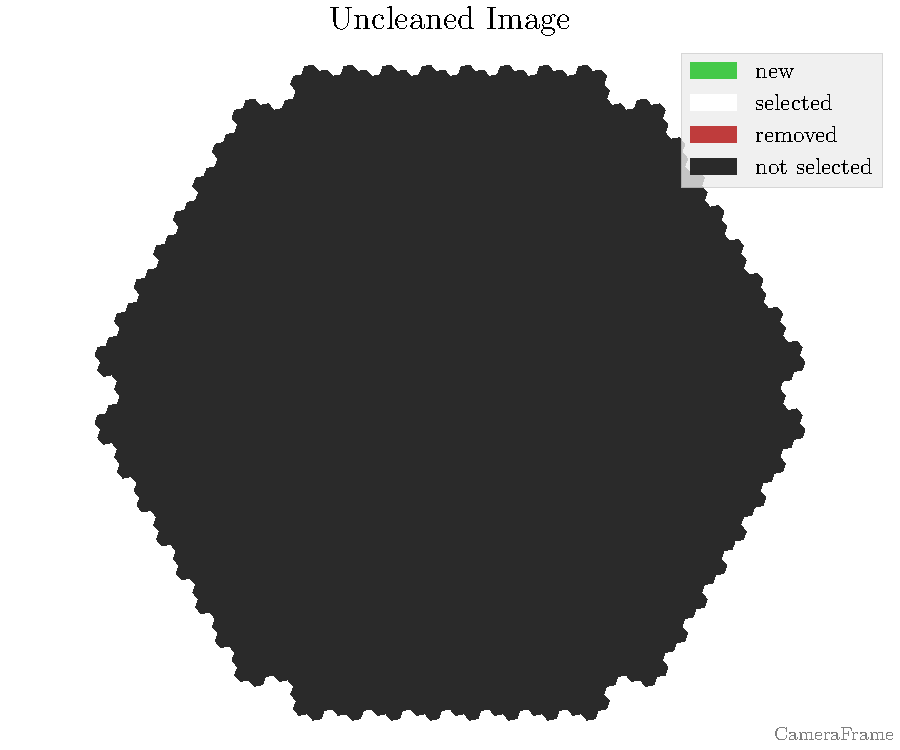
\includegraphics[width=\textwidth]{plots/cleaner_steps/light/null_image.pdf}
      }
      \only<4>{
        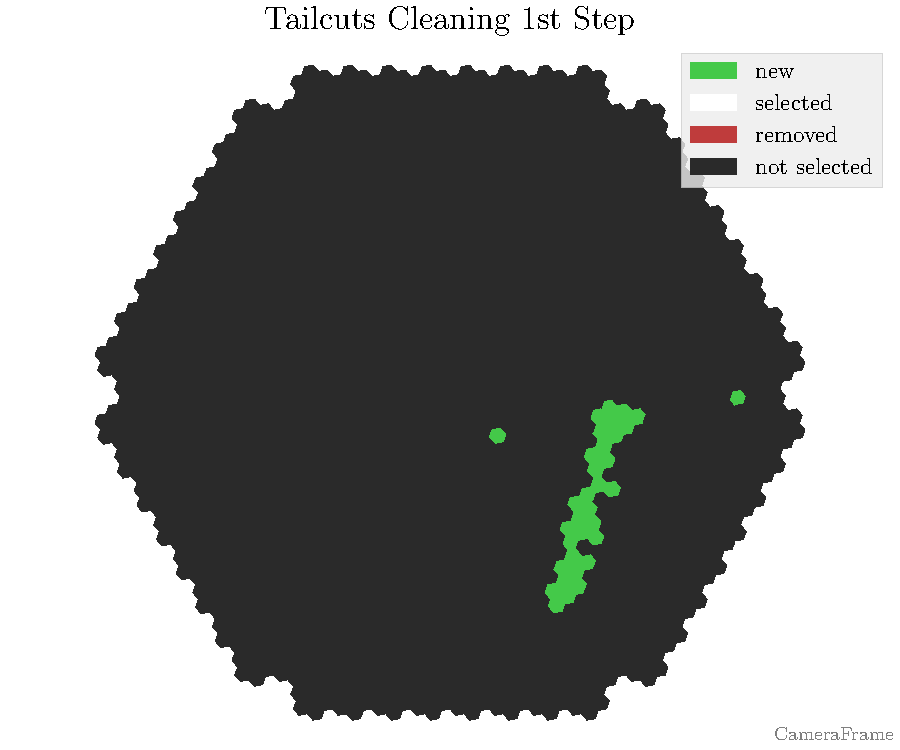
\includegraphics[width=\textwidth]{plots/cleaner_steps/light/tail_1.pdf}
      }
      \only<5>{
        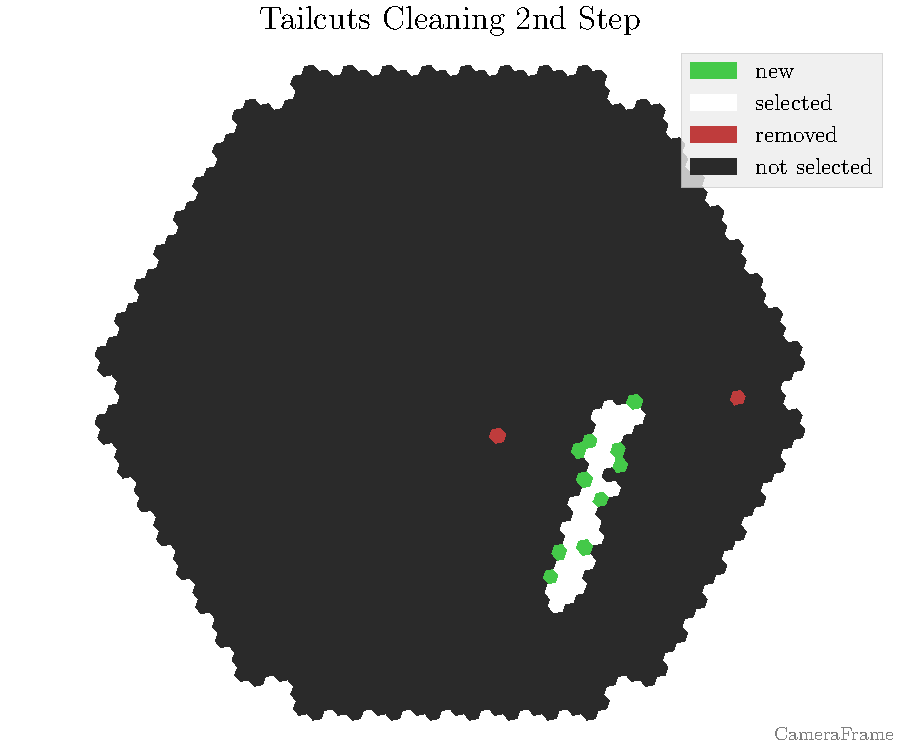
\includegraphics[width=\textwidth]{plots/cleaner_steps/light/tail_2.pdf}
      }
      \only<6>{
      \begin{itemize}
        \setlength\itemsep{1em}
        \item \code{darkgray!50!white}{TailcutsImageCleaner}
        \item \code{darkgray}{MARSImageCleaner}
        \item \code{darkgray!50!white}{FACTImageCleaner}
        \item \code{darkgray!50!white}{TimeConstrainedImageCleaner}
      \end{itemize}
      }
      \only<7>{
        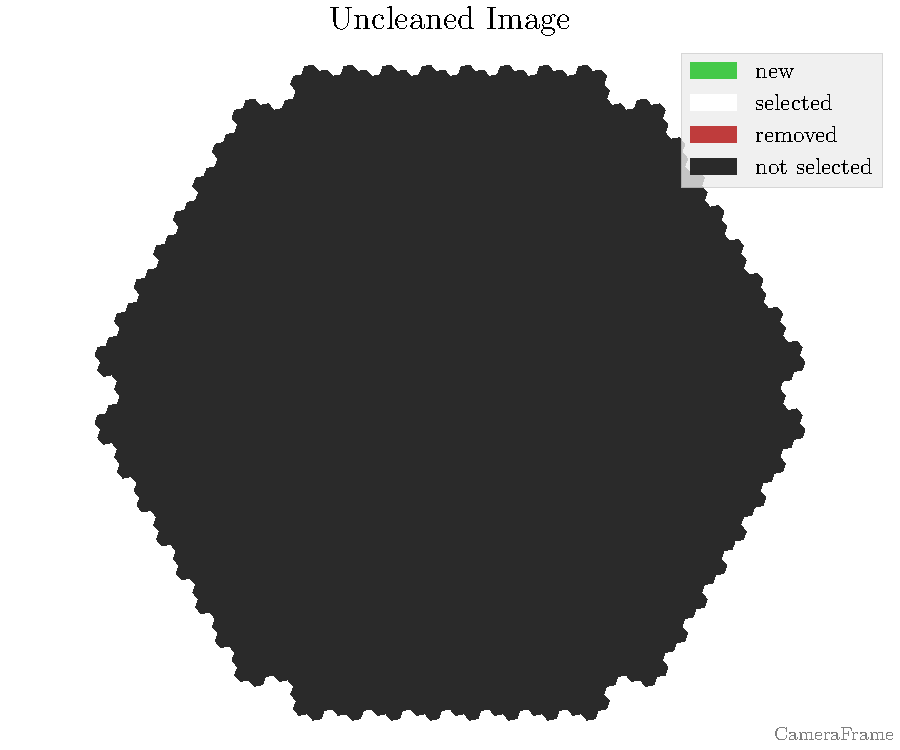
\includegraphics[width=\textwidth]{plots/cleaner_steps/light/null_image.pdf}
      }
      \only<8>{
        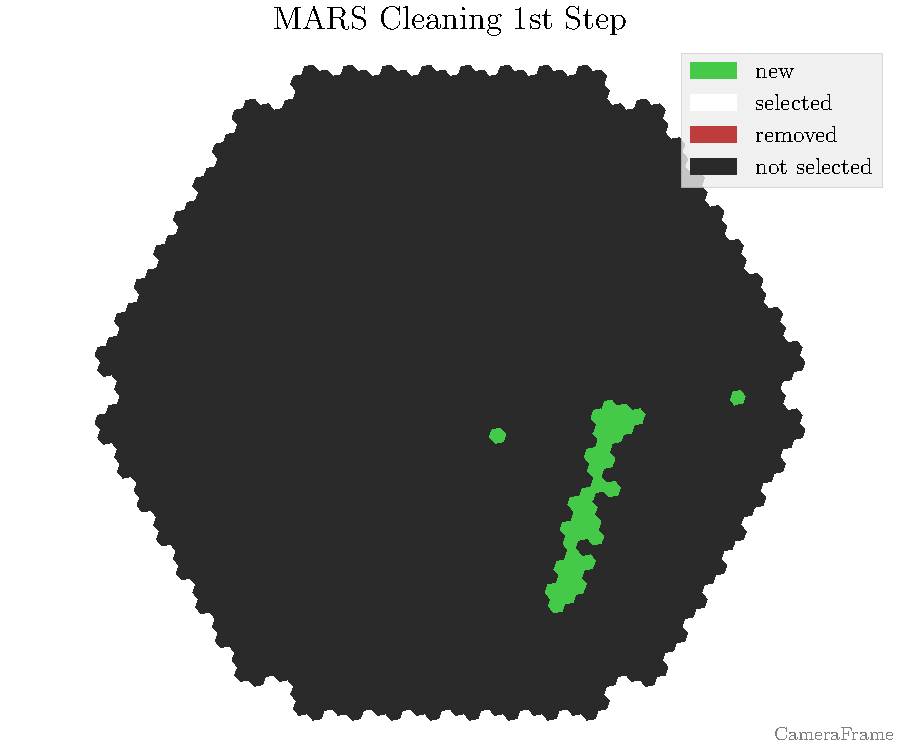
\includegraphics[width=\textwidth]{plots/cleaner_steps/light/mars_1.pdf}
      }
      \only<9>{
        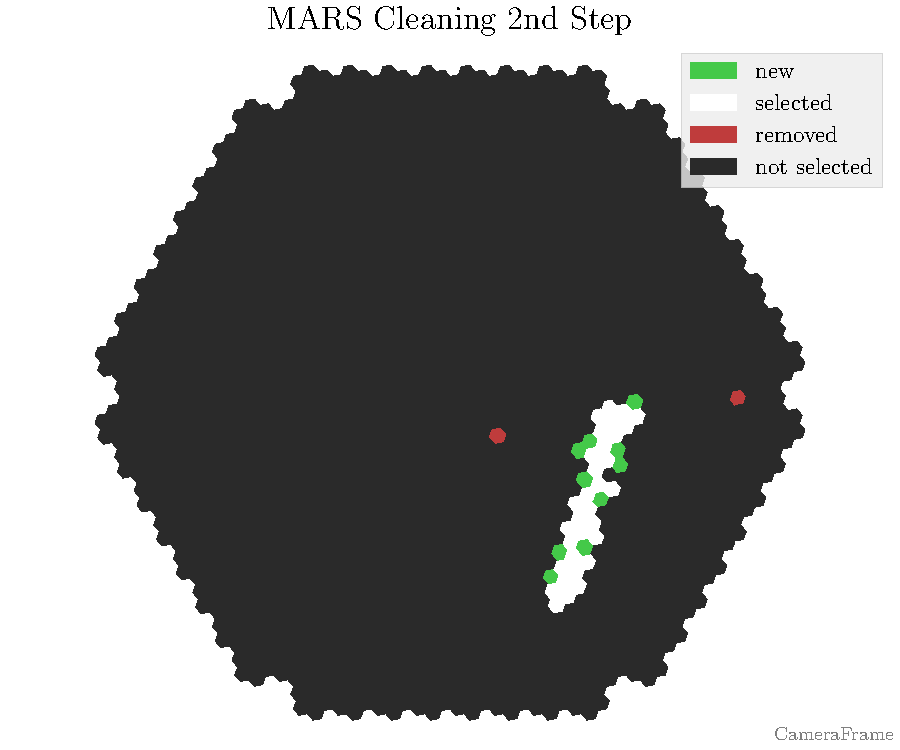
\includegraphics[width=\textwidth]{plots/cleaner_steps/light/mars_2.pdf}
      }
      \only<10>{
        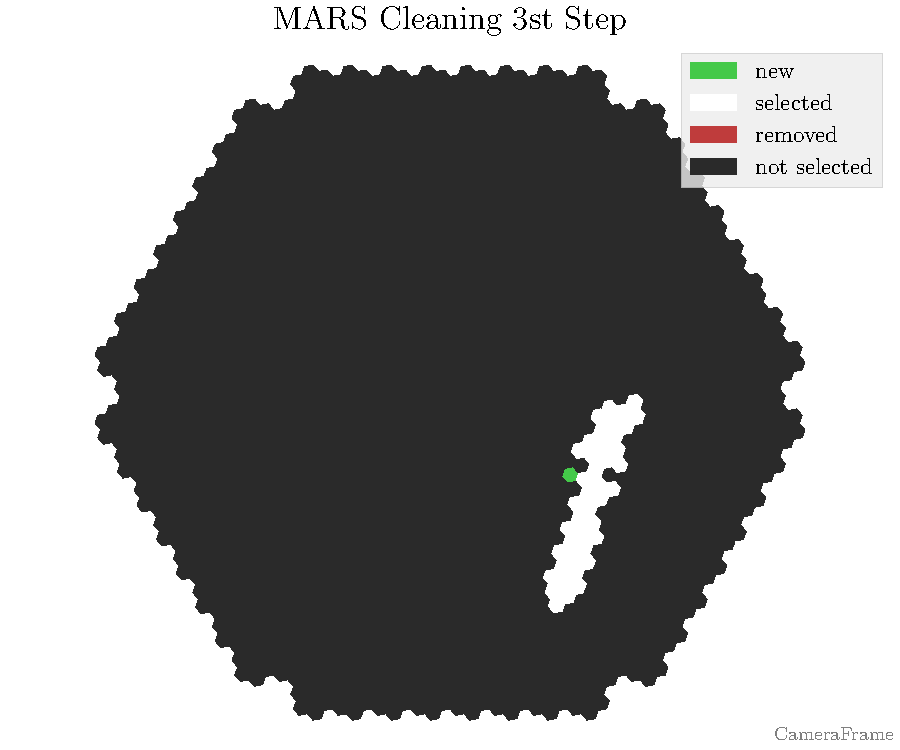
\includegraphics[width=\textwidth]{plots/cleaner_steps/light/mars_3.pdf}
      }
      \only<11>{
      \begin{itemize}
        \setlength\itemsep{1em}
        \item \code{darkgray!50!white}{TailcutsImageCleaner}
        \item \code{darkgray!50!white}{MARSImageCleaner}
        \item \code{darkgray}{FACTImageCleaner}
        \item \code{darkgray!50!white}{TimeConstrainedImageCleaner}
      \end{itemize}
      }
      \only<12>{
        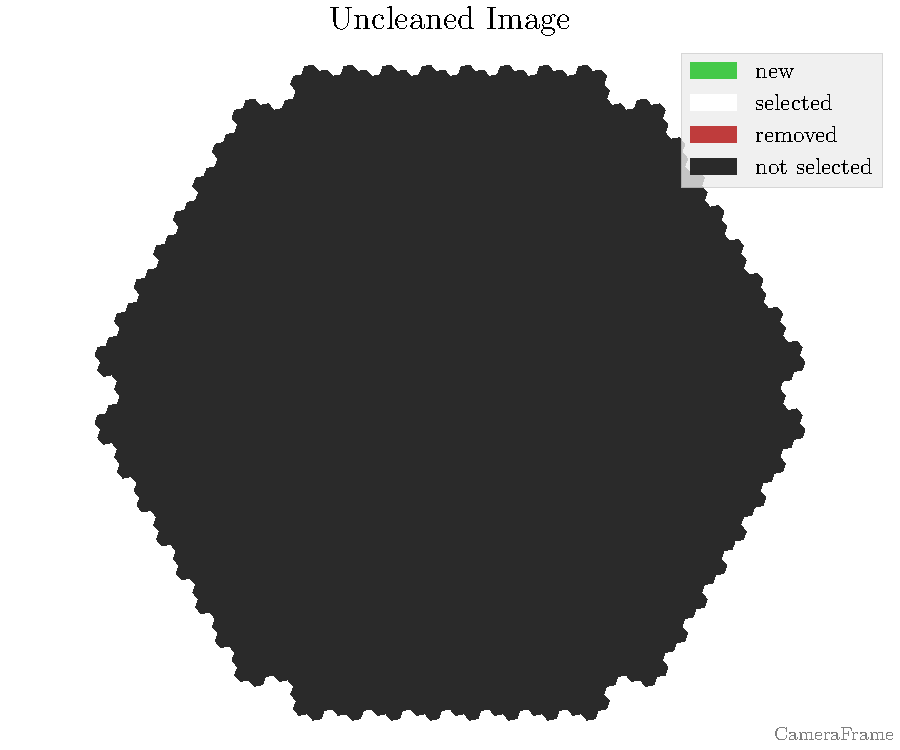
\includegraphics[width=\textwidth]{plots/cleaner_steps/light/null_image.pdf}
      }
      \only<13>{
        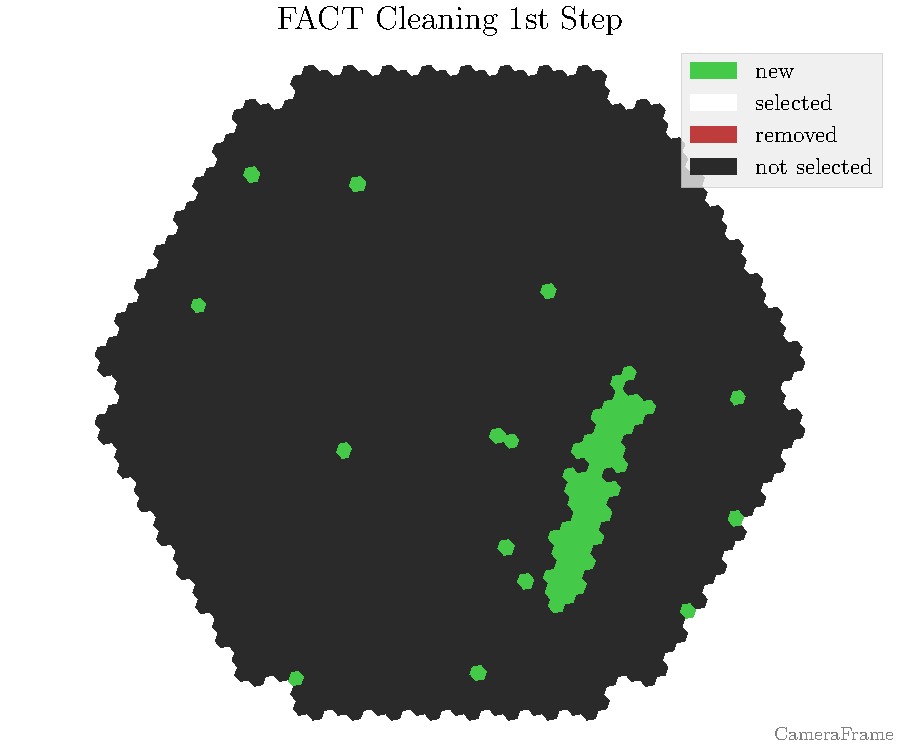
\includegraphics[width=\textwidth]{plots/cleaner_steps/light/fact_1.pdf}
      }
      \only<14>{
        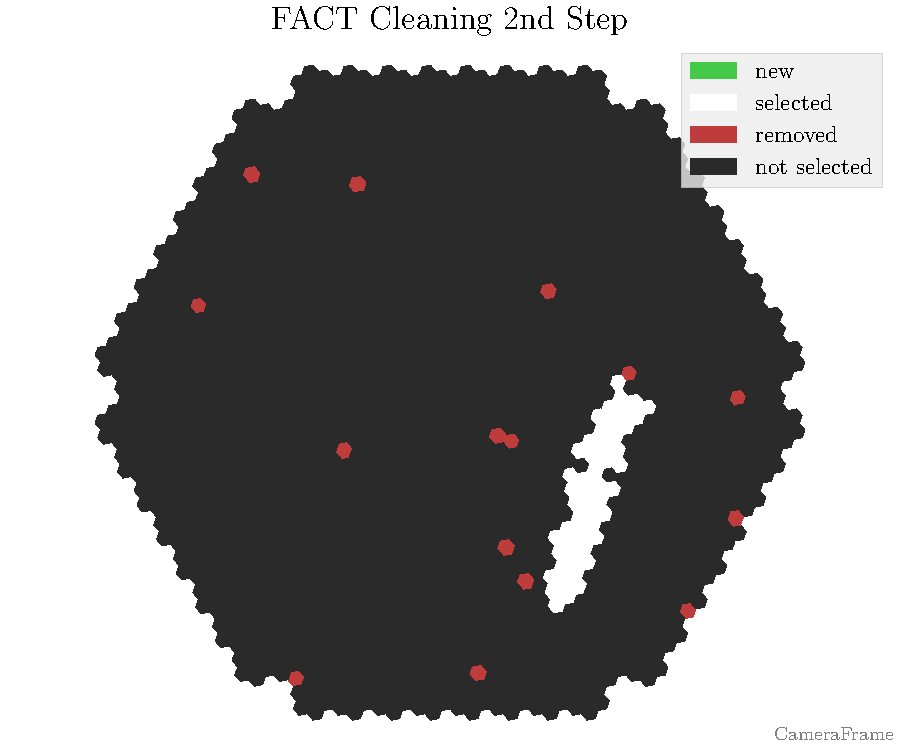
\includegraphics[width=\textwidth]{plots/cleaner_steps/light/fact_2.pdf}
      }
      \only<15>{
        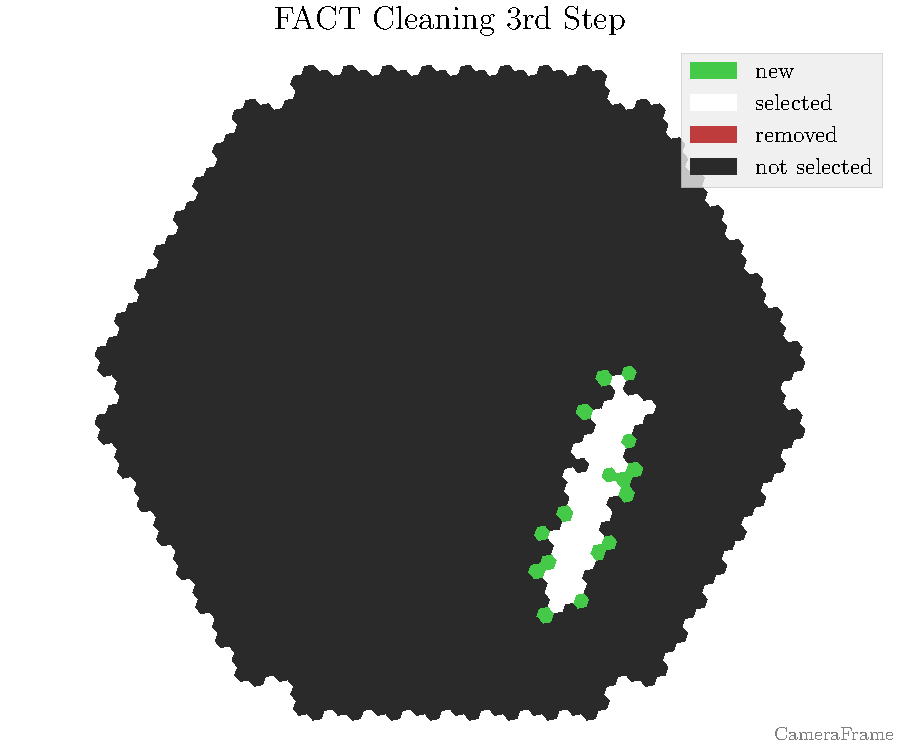
\includegraphics[width=\textwidth]{plots/cleaner_steps/light/fact_3.pdf}
      }
      \only<16>{
        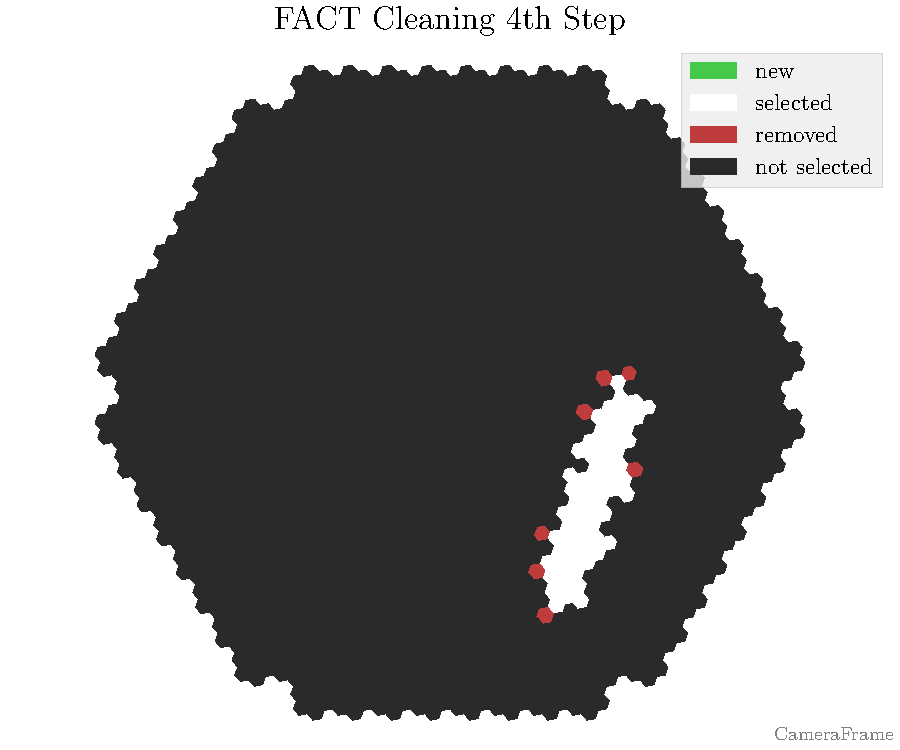
\includegraphics[width=\textwidth]{plots/cleaner_steps/light/fact_4.pdf}
      }
      \only<17>{
        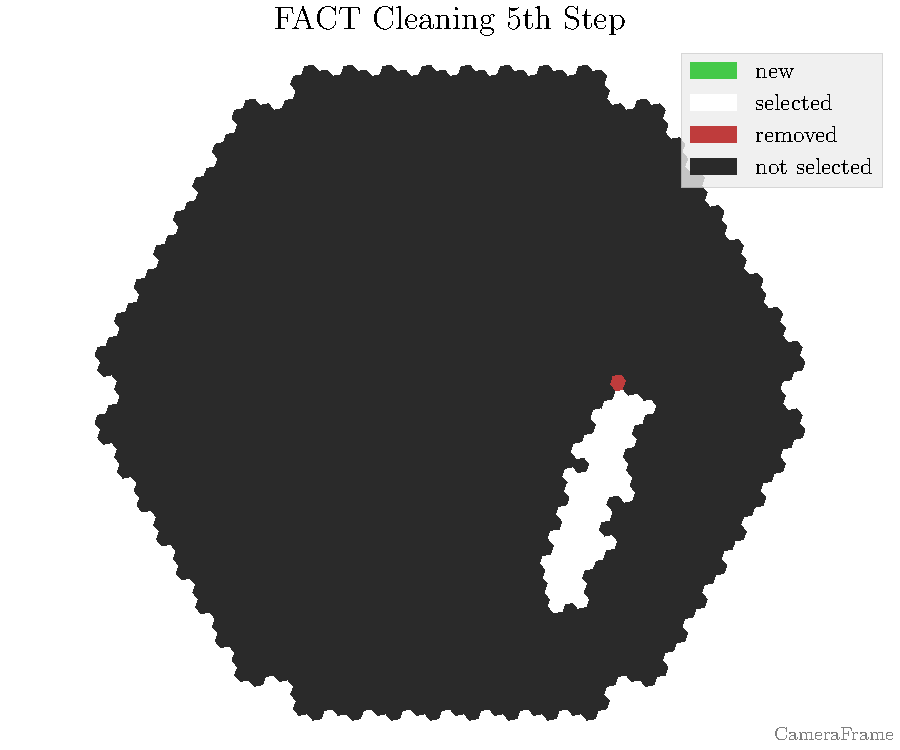
\includegraphics[width=\textwidth]{plots/cleaner_steps/light/fact_5.pdf}
      }
      \only<18>{
        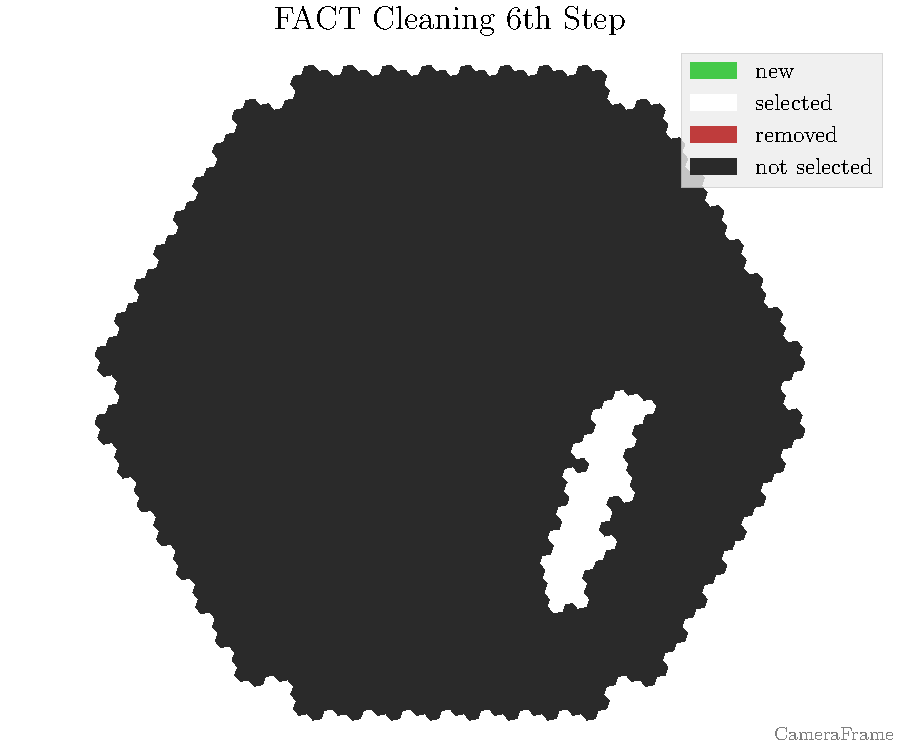
\includegraphics[width=\textwidth]{plots/cleaner_steps/light/fact_6.pdf}
      }
      \only<19>{
      \begin{itemize}
        \setlength\itemsep{1em}
        \item \code{darkgray!50!white}{TailcutsImageCleaner}
        \item \code{darkgray!50!white}{MARSImageCleaner}
        \item \code{darkgray!50!white}{FACTImageCleaner}
        \item \code{darkgray}{TimeConstrainedImageCleaner}
      \end{itemize}
      }
      \only<20>{
        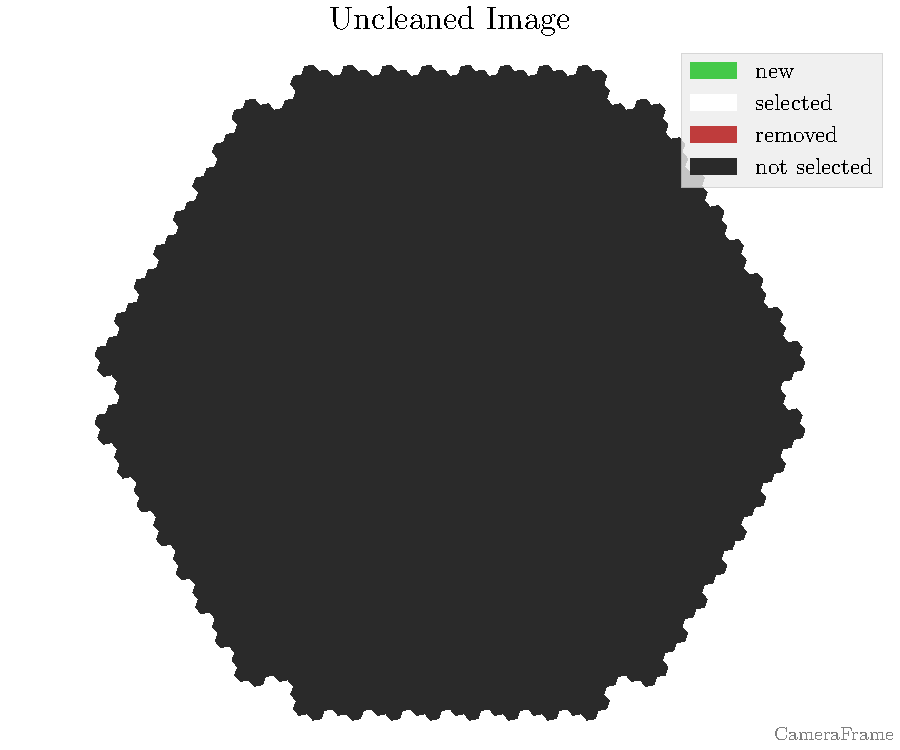
\includegraphics[width=\textwidth]{plots/cleaner_steps/light/null_image.pdf}
      }
      \only<21>{
        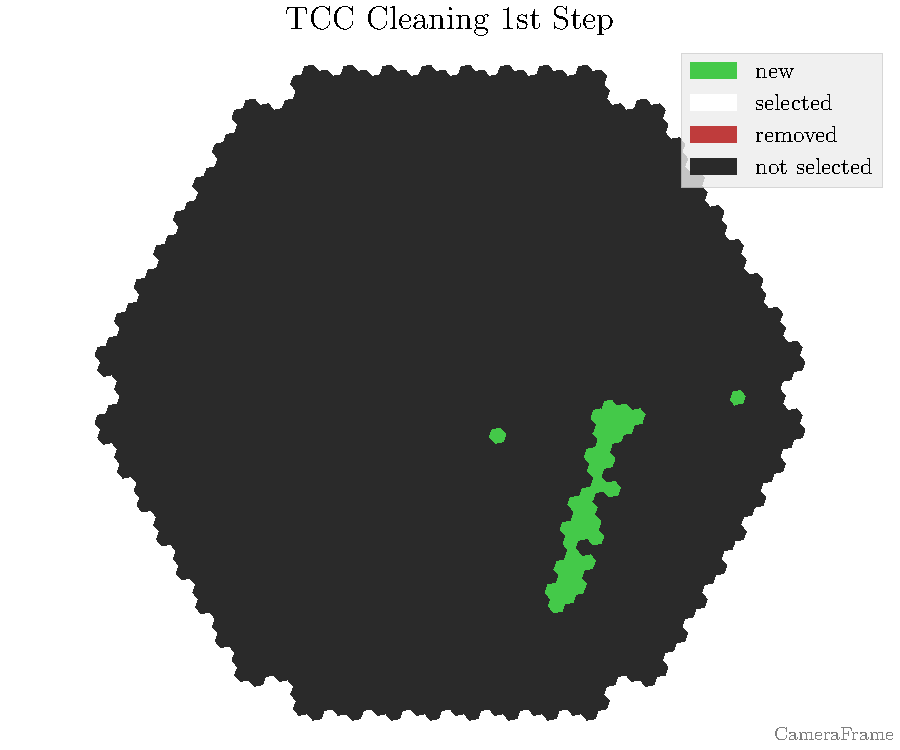
\includegraphics[width=\textwidth]{plots/cleaner_steps/light/tcc_1.pdf}
      }
      \only<22>{
        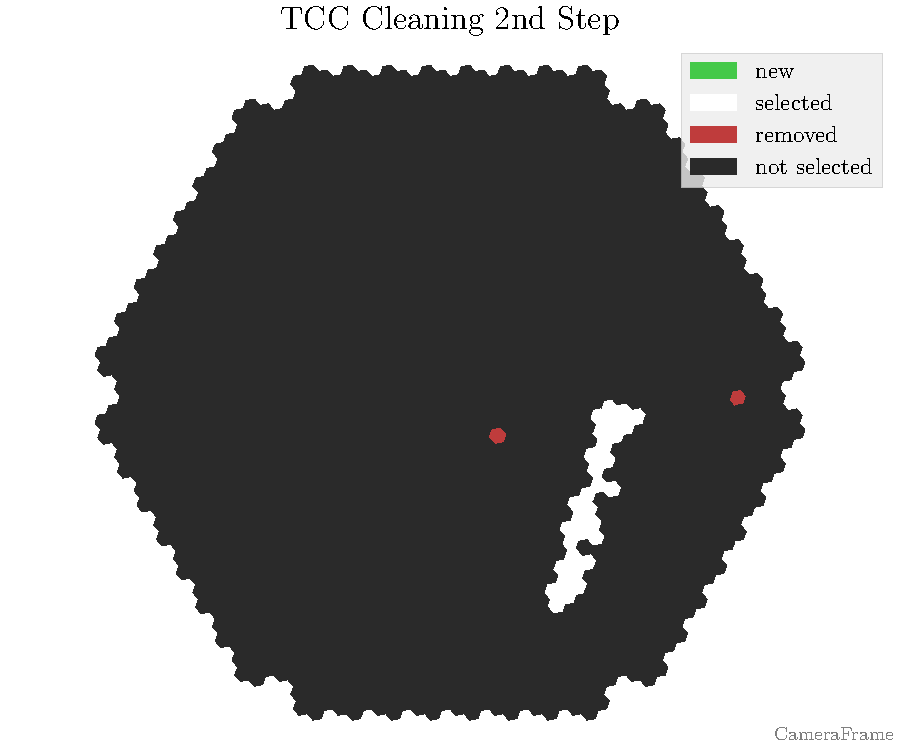
\includegraphics[width=\textwidth]{plots/cleaner_steps/light/tcc_2.pdf}
      }
      \only<23>{
        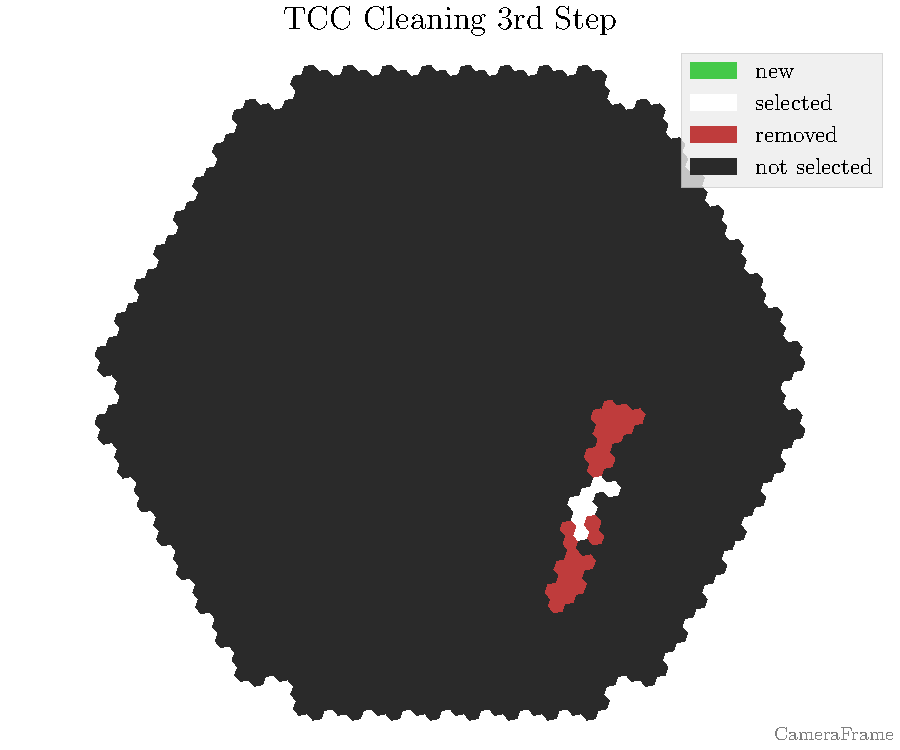
\includegraphics[width=\textwidth]{plots/cleaner_steps/light/tcc_3.pdf}
      }
      \only<24>{
        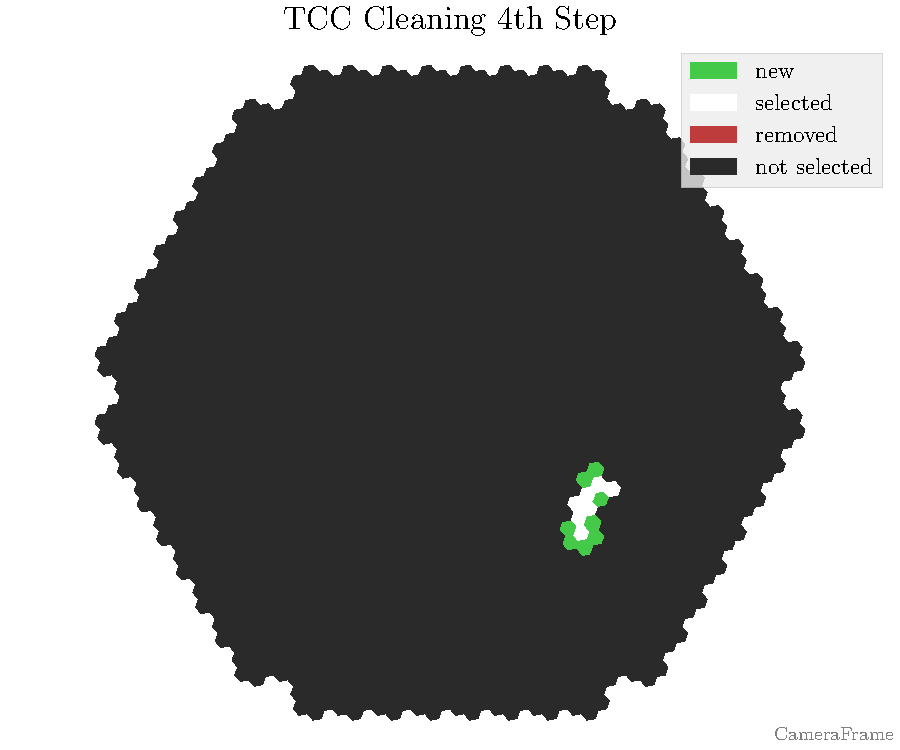
\includegraphics[width=\textwidth]{plots/cleaner_steps/light/tcc_4.pdf}
      }
      \only<25>{
        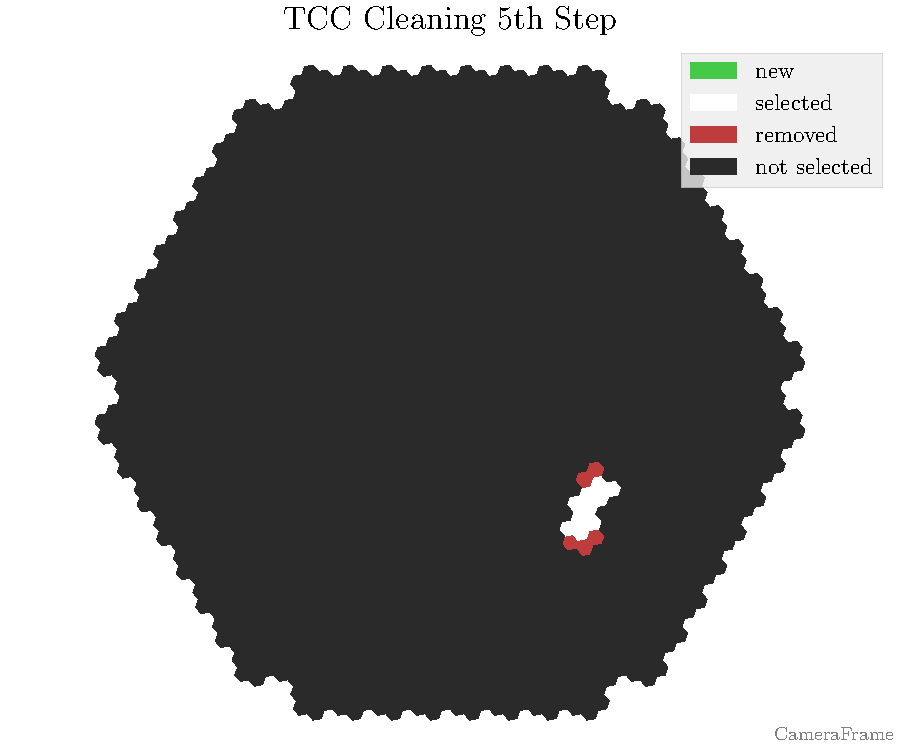
\includegraphics[width=\textwidth]{plots/cleaner_steps/light/tcc_5.pdf}
      }
    \end{overlayarea}
    }
    \raisebox{10ex}{
    \begin{overlayarea}{0.58\textwidth}{3.5cm}
      \only<1>{
        \centering
        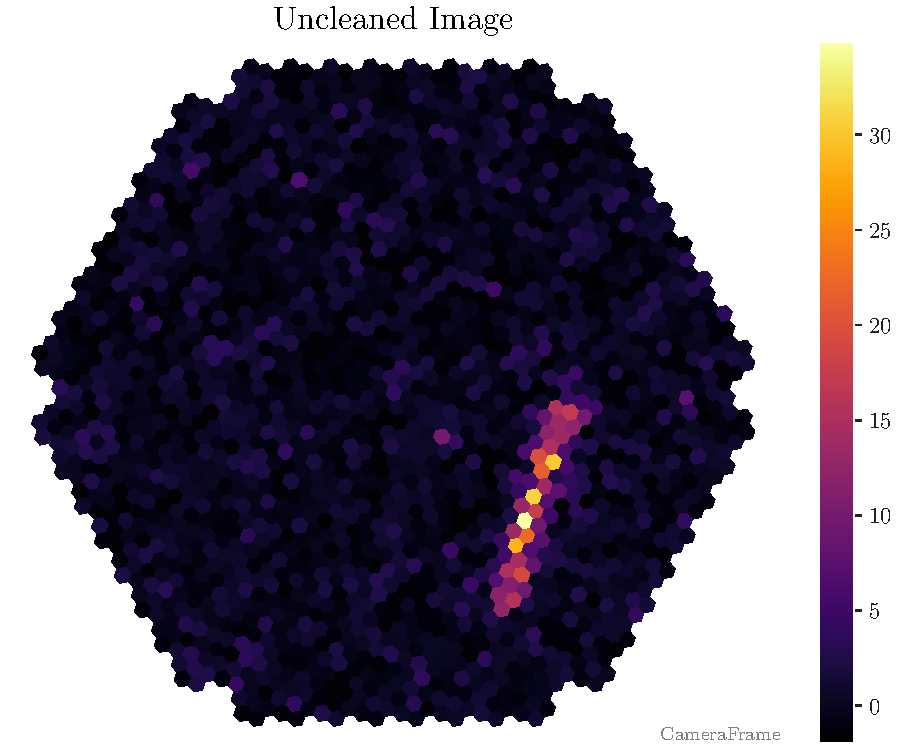
\includegraphics[width=0.65\textwidth]{plots/cleaner_steps/light/uncleaned_image.pdf}
      }
      \only<2>{
      \begin{enumerate}%TailcutsImageCleaner
        \item Select pixels that pass the \code{darkgray!70!white}{core threshold} (this talk: \(\SI{7}{\pe}\))
        \item Add pixels that pass the \code{darkgray!70!white}{boundary threshold} (here: \(\SI{5}{\pe}\))
      \end{enumerate}
      }
      \only<3>{
      \begin{enumerate}%TailcutsImageCleaner
        \item \textcolor{darkgray!50!white}{Select pixels that pass the \code{darkgray!35!white}{core threshold} (this talk: \(\SI{7}{\pe}\))}
        \item \textcolor{darkgray!50!white}{Add pixels that pass the \code{darkgray!35!white}{boundary threshold} (here: \(\SI{5}{\pe}\))}
      \end{enumerate}
      }
      \only<4>{
      \begin{enumerate}%TailcutsImageCleaner
        \item Select pixels that pass the \code{darkgray!70!white}{core threshold} (this talk: \(\SI{7}{\pe}\))
        \item \textcolor{darkgray!50!white}{Add pixels that pass the \code{darkgray!35!white}{boundary threshold} (here: \(\SI{5}{\pe}\))}
      \end{enumerate}
      }
      \only<5>{
      \begin{enumerate}%TailcutsImageCleaner
        \item \textcolor{darkgray!50!white}{Select pixels that pass the \code{darkgray!35!white}{core threshold} (this talk: \(\SI{7}{\pe}\))}
        \item Add pixels that pass the \code{darkgray!70!white}{boundary threshold} (here: \(\SI{5}{\pe}\))
      \end{enumerate}
      }

      \only<6>{
      \begin{enumerate}%MARSImageCleaner
        \item Select pixels that pass the \code{darkgray!70!white}{core} and \code{darkgray!70!white}{boundary threshold}, analogous to \code{darkgray!70!white}{TailcutsImageCleaner}
        \item Add pixels that are a neighbor of a neighbor of a core pixel, if they are above the \code{darkgray!70!white}{boundary threshold}
      \end{enumerate}
      }
      \only<7>{
      \begin{enumerate}%MARSImageCleaner
        \item \textcolor{darkgray!50!white}{Select pixels that pass the \code{darkgray!35!white}{core} and \code{darkgray!35!white}{boundary threshold}, analogous to \code{darkgray!35!white}{TailcutsImageCleaner}}
        \item \textcolor{darkgray!50!white}{Add pixels that are a neighbor of a neighbor of a core pixel, if they are above the \code{darkgray!35!white}{boundary threshold}}
      \end{enumerate}
      }
      \only<8-9>{
      \begin{enumerate}%MARSImageCleaner
        \item Select pixels that pass the \code{darkgray!70!white}{core} and \code{darkgray!70!white}{boundary threshold}, analogous to \code{darkgray!70!white}{TailcutsImageCleaner}
        \item \textcolor{darkgray!50!white}{Add pixels that are a neighbor of a neighbor of a core pixel, if they are above the \code{darkgray!35!white}{boundary threshold}}
      \end{enumerate}
      }
      \only<10>{
      \begin{enumerate}%MARSImageCleaner
        \item \textcolor{darkgray!50!white}{Select pixels that pass the \code{darkgray!35!white}{core} and \code{darkgray!35!white}{boundary threshold}, analogous to \code{darkgray!35!white}{TailcutsImageCleaner}}
        \item Add pixels that are a neighbor of a neighbor of a core pixel, if they are above the \code{darkgray!70!white}{boundary threshold}
      \end{enumerate}
      }
      \only<11>{
      \begin{enumerate}%FACTImageCleaner
        \item Find all pixels that contain more photons than the \code{darkgray!70!white}{core threshold} (this talk: \(\SI{4}{\pe}\))
        \item Remove pixels with less than \(N\) neighbors (this talk: \(N=2\))
        \item Add remaining neighbors that are above the \code{darkgray!70!white}{boundary threshold} (this talk: \(\SI{2}{\pe}\))
        \item Remove pixels that have less than \(N\) neighbors, that arrive within a given timeframe (here: \SI{5}{\nano\second})
        \item Remove pixels that have less than \(N\) neighbors
        \item Remove pixels that have less than \(N\) neighbors, arriving within a given timeframe (same as in step 4)
      \end{enumerate}
      }
      \only<12>{
      \begin{enumerate}%FACTImageCleaner
        \item \textcolor{darkgray!50!white}{Find all pixels that contain more photons than the \code{darkgray!35!white}{core threshold} (this talk: \(\SI{4}{\pe}\))}
        \item \textcolor{darkgray!50!white}{Remove pixels with less than \(N\) neighbors (this talk: \(N=2\))}
        \item \textcolor{darkgray!50!white}{Add remaining neighbors that are above the \code{darkgray!35!white}{boundary threshold} (this talk: \(\SI{2}{\pe}\))}
        \item \textcolor{darkgray!50!white}{Remove pixels that have less than \(N\) neighbors, that arrive within a given timeframe (here: \SI{5}{\nano\second})}
        \item \textcolor{darkgray!50!white}{Remove pixels that have less than \(N\) neighbors}
        \item \textcolor{darkgray!50!white}{Remove pixels that have less than \(N\) neighbors, arriving within a given timeframe (same as in step 4)}
      \end{enumerate}
      }
      \only<13>{
      \begin{enumerate}%FACTImageCleaner
        \item Find all pixels that contain more photons than the \code{darkgray!70!white}{core threshold} (this talk: \(\SI{4}{\pe}\))
        \item \textcolor{darkgray!50!white}{Remove pixels with less than \(N\) neighbors (this talk: \(N=2\))}
        \item \textcolor{darkgray!50!white}{Add remaining neighbors that are above the \code{darkgray!35!white}{boundary threshold} (this talk: \(\SI{2}{\pe}\))}
        \item \textcolor{darkgray!50!white}{Remove pixels that have less than \(N\) neighbors, that arrive within a given timeframe (here: \SI{5}{\nano\second})}
        \item \textcolor{darkgray!50!white}{Remove pixels that have less than \(N\) neighbors}
        \item \textcolor{darkgray!50!white}{Remove pixels that have less than \(N\) neighbors, arriving within a given timeframe (same as in step 4)}
      \end{enumerate}
      }
      \only<14>{
      \begin{enumerate}%FACTImageCleaner
        \item \textcolor{darkgray!50!white}{Find all pixels that contain more photons than the \code{darkgray!35!white}{core threshold} (this talk: \(\SI{4}{\pe}\))}
        \item Remove pixels with less than \(N\) neighbors (this talk: \(N=2\))
        \item \textcolor{darkgray!50!white}{Add remaining neighbors that are above the \code{darkgray!35!white}{boundary threshold} (this talk: \(\SI{2}{\pe}\))}
        \item \textcolor{darkgray!50!white}{Remove pixels that have less than \(N\) neighbors, that arrive within a given timeframe (here: \SI{5}{\nano\second})}
        \item \textcolor{darkgray!50!white}{Remove pixels that have less than \(N\) neighbors}
        \item \textcolor{darkgray!50!white}{Remove pixels that have less than \(N\) neighbors, arriving within a given timeframe (same as in step 4)}
      \end{enumerate}
      }
      \only<15>{
      \begin{enumerate}%FACTImageCleaner
        \item \textcolor{darkgray!50!white}{Find all pixels that contain more photons than the \code{darkgray!35!white}{core threshold} (this talk: \(\SI{4}{\pe}\))}
        \item \textcolor{darkgray!50!white}{Remove pixels with less than \(N\) neighbors (this talk: \(N=2\))}
        \item Add remaining neighbors that are above the \code{darkgray!70!white}{boundary threshold} (this talk: \(\SI{2}{\pe}\))
        \item \textcolor{darkgray!50!white}{Remove pixels that have less than \(N\) neighbors, that arrive within a given timeframe (here: \SI{5}{\nano\second})}
        \item \textcolor{darkgray!50!white}{Remove pixels that have less than \(N\) neighbors}
        \item \textcolor{darkgray!50!white}{Remove pixels that have less than \(N\) neighbors, arriving within a given timeframe (same as in step 4)}
      \end{enumerate}
      }
      \only<16>{
      \begin{enumerate}%FACTImageCleaner
        \item \textcolor{darkgray!50!white}{Find all pixels that contain more photons than the \code{darkgray!35!white}{core threshold} (this talk: \(\SI{4}{\pe}\))}
        \item \textcolor{darkgray!50!white}{Remove pixels with less than \(N\) neighbors (this talk: \(N=2\))}
        \item \textcolor{darkgray!50!white}{Add remaining neighbors that are above the \code{darkgray!35!white}{boundary threshold} (this talk: \(\SI{2}{\pe}\))}
        \item Remove pixels that have less than \(N\) neighbors, that arrive within a given timeframe (here: \SI{5}{\nano\second})
        \item \textcolor{darkgray!50!white}{Remove pixels that have less than \(N\) neighbors}
        \item \textcolor{darkgray!50!white}{Remove pixels that have less than \(N\) neighbors, arriving within a given timeframe (same as in step 4)}
      \end{enumerate}
      }
      \only<17>{
      \begin{enumerate}%FACTImageCleaner
        \item \textcolor{darkgray!50!white}{Find all pixels that contain more photons than the \code{darkgray!35!white}{core threshold} (this talk: \(\SI{4}{\pe}\))}
        \item \textcolor{darkgray!50!white}{Remove pixels with less than \(N\) neighbors (this talk: \(N=2\))}
        \item \textcolor{darkgray!50!white}{Add remaining neighbors that are above the \code{darkgray!35!white}{boundary threshold} (this talk: \(\SI{2}{\pe}\))}
        \item \textcolor{darkgray!50!white}{Remove pixels that have less than \(N\) neighbors, that arrive within a given timeframe (here: \SI{5}{\nano\second})}
        \item Remove pixels that have less than \(N\) neighbors
        \item \textcolor{darkgray!50!white}{Remove pixels that have less than \(N\) neighbors, arriving within a given timeframe (same as in step 4)}
      \end{enumerate}
      }
      \only<18>{
      \begin{enumerate}%FACTImageCleaner
        \item \textcolor{darkgray!50!white}{Find all pixels that contain more photons than the \code{darkgray!35!white}{core threshold} (this talk: \(\SI{4}{\pe}\))}
        \item \textcolor{darkgray!50!white}{Remove pixels with less than \(N\) neighbors (this talk: \(N=2\))}
        \item \textcolor{darkgray!50!white}{Add remaining neighbors that are above the \code{darkgray!35!white}{boundary threshold} (this talk: \(\SI{2}{\pe}\))}
        \item \textcolor{darkgray!50!white}{Remove pixels that have less than \(N\) neighbors, that arrive within a given timeframe (here: \SI{5}{\nano\second})}
        \item \textcolor{darkgray!50!white}{Remove pixels that have less than \(N\) neighbors}
        \item Remove pixels that have less than \(N\) neighbors, arriving within the given timeframe (same as in step 4)
      \end{enumerate}
      }
      \only<19>{
      \begin{enumerate}%TimeConstrainedImageCleaner
        \item Find all core pixels above the \code{darkgray!70!white}{core threshold} (this talk: \(\SI{7}{\pe}\))
        \item Remove pixels with less than \(N\) neighbors (this talk: \(N=1\))
        \item Keep all pixels that arrive within a time limit of the average arrival time (\code{darkgray!70!white}{time_limit_core}: \SI{4.5}{\nano\second})
        \item Find all neighboring pixels above the \code{darkgray!70!white}{boundary threshold} (this talk: \(\SI{5}{\pe}\))
        \item Remove all pixels with less than \(N\) neighbors arriving within a given timeframe (\code{darkgray!70!white}{time_limit_boundary}: \SI{1.5}{\nano\second})
      \end{enumerate}
      }
      \only<20>{
      \begin{enumerate}%TimeConstrainedImageCleaner
        \item \textcolor{darkgray!50!white}{Find all core pixels above the \code{darkgray!35!white}{core threshold} (this talk: \(\SI{7}{\pe}\))}
        \item \textcolor{darkgray!50!white}{Remove pixels with less than \(N\) neighbors (this talk: \(N=1\))}
        \item \textcolor{darkgray!50!white}{Keep all pixels that arrive within a time limit of the average arrival time (\code{darkgray!35!white}{time_limit_core}: \SI{4.5}{\nano\second})}
        \item \textcolor{darkgray!50!white}{Find all neighboring pixels above the \code{darkgray!35!white}{boundary threshold} (this talk: \(\SI{5}{\pe}\))}
        \item \textcolor{darkgray!50!white}{Remove all pixels with less than \(N\) neighbors arriving within a given timeframe (\code{darkgray!35!white}{time_limit_boundary}: \SI{1.5}{\nano\second})}
      \end{enumerate}
      }
      \only<21>{
      \begin{enumerate}%TimeConstrainedImageCleaner
        \item Find all core pixels above the \code{darkgray!70!white}{core threshold} (this talk: \(\SI{7}{\pe}\))
        \item \textcolor{darkgray!50!white}{Remove pixels with less than \(N\) neighbors (this talk: \(N=1\))}
        \item \textcolor{darkgray!50!white}{Keep all pixels that arrive within a time limit of the average arrival time (\code{darkgray!35!white}{time_limit_core}: \SI{4.5}{\nano\second})}
        \item \textcolor{darkgray!50!white}{Find all neighboring pixels above the \code{darkgray!35!white}{boundary threshold} (this talk: \(\SI{5}{\pe}\))}
        \item \textcolor{darkgray!50!white}{Remove all pixels with less than \(N\) neighbors arriving within a given timeframe (\code{darkgray!35!white}{time_limit_boundary}: \SI{1.5}{\nano\second})}
      \end{enumerate}
      }
      \only<22>{
      \begin{enumerate}%TimeConstrainedImageCleaner
        \item \textcolor{darkgray!50!white}{Find all core pixels above the \code{darkgray!35!white}{core threshold} (this talk: \(\SI{7}{\pe}\))}
        \item Remove pixels with less than \(N\) neighbors (this talk: \(N=1\))
        \item \textcolor{darkgray!50!white}{Keep all pixels that arrive within a time limit of the average arrival time (\code{darkgray!35!white}{time_limit_core}: \SI{4.5}{\nano\second})}
        \item \textcolor{darkgray!50!white}{Find all neighboring pixels above the \code{darkgray!35!white}{boundary threshold} (this talk: \(\SI{5}{\pe}\))}
        \item \textcolor{darkgray!50!white}{Remove all pixels with less than \(N\) neighbors arriving within a given timeframe (\code{darkgray!35!white}{time_limit_boundary}: \SI{1.5}{\nano\second})}
      \end{enumerate}
      }
      \only<23>{
      \begin{enumerate}%TimeConstrainedImageCleaner
        \item \textcolor{darkgray!50!white}{Find all core pixels above the \code{darkgray!35!white}{core threshold} (this talk: \(\SI{7}{\pe}\))}
        \item \textcolor{darkgray!50!white}{Remove pixels with less than \(N\) neighbors (this talk: \(N=1\))}
        \item Keep all pixels that arrive within a time limit of the average arrival time (\code{darkgray!70!white}{time_limit_core}: \SI{4.5}{\nano\second})
        \item \textcolor{darkgray!50!white}{Find all neighboring pixels above the \code{darkgray!35!white}{boundary threshold} (this talk: \(\SI{5}{\pe}\))}
        \item \textcolor{darkgray!50!white}{Remove all pixels with less than \(N\) neighbors arriving within a given timeframe (\code{darkgray!35!white}{time_limit_boundary}: \SI{1.5}{\nano\second})}
      \end{enumerate}
      }
      \only<24>{
      \begin{enumerate}%TimeConstrainedImageCleaner
        \item \textcolor{darkgray!50!white}{Find all core pixels above the \code{darkgray!35!white}{core threshold} (this talk: \(\SI{7}{\pe}\))}
        \item \textcolor{darkgray!50!white}{Remove pixels with less than \(N\) neighbors (this talk: \(N=1\))}
        \item \textcolor{darkgray!50!white}{Keep all pixels that arrive within a time limit of the average arrival time (\code{darkgray!35!white}{time_limit_core}: \SI{4.5}{\nano\second})}
        \item Find all neighboring pixels above the \code{darkgray!70!white}{boundary threshold} (this talk: \(\SI{5}{\pe}\))
        \item \textcolor{darkgray!50!white}{Remove all pixels with less than \(N\) neighbors arriving within a given timeframe (\code{darkgray!35!white}{time_limit_boundary}: \SI{1.5}{\nano\second})}
      \end{enumerate}
      }
      \only<25>{
      \begin{enumerate}%TimeConstrainedImageCleaner
        \item \textcolor{darkgray!50!white}{Find all core pixels above the \code{darkgray!35!white}{core threshold} (this talk: \(\SI{7}{\pe}\))}
        \item \textcolor{darkgray!50!white}{Remove pixels with less than \(N\) neighbors (this talk: \(N=1\))}
        \item \textcolor{darkgray!50!white}{Keep all pixels that arrive within a time limit of the average arrival time (\code{darkgray!35!white}{time_limit_core}: \SI{4.5}{\nano\second})}
        \item \textcolor{darkgray!50!white}{Find all neighboring pixels above the \code{darkgray!35!white}{boundary threshold} (this talk: \(\SI{5}{\pe}\))}
        \item Remove all pixels with less than \(N\) neighbors arriving within a given timeframe (\code{darkgray!70!white}{time_limit_boundary}: \SI{1.5}{\nano\second})
      \end{enumerate}
      }
    \end{overlayarea}
    }
  \end{frame}
    }

\subsection{Hyperparameters}%
\label{sub:Hyperparameters}
\begin{frame}[t]{Choosing reasonable hyperparameters for the grid search}
    % \todo[inline]{might need to think more about the layout of this slide}
    \begin{overlayarea}{\textwidth}{2.3cm}
        \begin{itemize}
            \item<1-> Begin by calculating core thresholds from quantiles for a given telescope type
            \item<3-> Select the boundary thresholds as ratios of the core thresholds (\eg 0.25, 0.33, 0.5\dots)
            \item<4-> Select feasible values for the number of neighbors (\eg 0, 1, 2, 3,\dots)
            \item<5-> Set reasonable time limits for the time-based algorithms
        \end{itemize}
        % \vspace{0.5cm}
    \end{overlayarea}
    \begin{overlayarea}{\textwidth}{\textheight}
        \only<2->{
            \ifthenelse{\equal{\theme}{\string 1}}
            {% use dark theme
            \vfill
            \centering
            \includegraphics[width=0.85\textwidth]{build/quantiles_plot_dark.pdf}
            }
            {% use light theme
            \vfill
            \centering
            \includegraphics[width=0.85\textwidth]{build/quantiles_plot_light.pdf}
            }
        }
    \end{overlayarea}
\end{frame}

\subsection{This Work's Pipeline}
\begin{frame}{This Work's Pipeline}
    \ifthenelse{\equal{\theme}{\string 1}}
    {% use dark theme
    \centering
    \includegraphics[width=\textwidth]{build/tikz/data_pipeline_dark.pdf}
    }
    {% use light theme
    \centering
    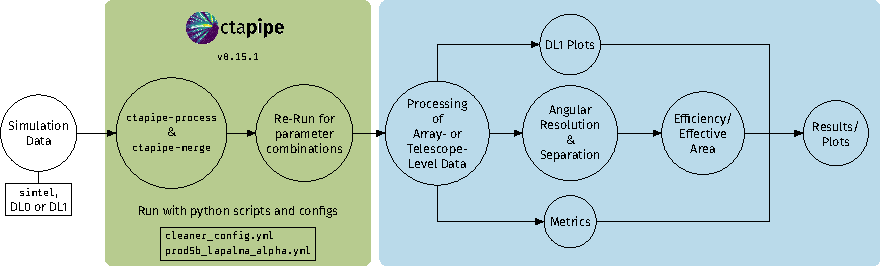
\includegraphics[width=\textwidth]{build/tikz/data_pipeline.pdf}
    }
\end{frame}
\subsection{Efficiency and Angular Resolution}%
\label{sub:Efficiency_AR}

\begin{frame}{Efficiency and Angular Resolution}
    \begin{equation*}
        \eff = \frac{n_\text{reco}}{n_\text{total}}
    \end{equation*}
    \begin{columns}
        \begin{column}{0.48\textwidth}
            \centering
            \includegraphics[height=0.8\textheight]{build/AR_Aeff_MST_0.10_0.15_dark.pdf}
        \end{column}
        \begin{column}{0.48\textwidth}
            \centering
            \includegraphics[height=0.8\textheight]{build/AR_Aeff_MST_0.40_0.45_dark.pdf}
        \end{column}
    \end{columns}
\end{frame}

\begin{frame}{Efficiency vs. Angular Resolution}
    \centering
    \includegraphics[width=0.75\textwidth]{build/ar_vs_eff_dark.pdf}
\end{frame}

\begin{frame}{Evaluation Metrics}
    \begin{minipage}{0.48\textwidth}
        \begin{align*}
            \tpr &= \frac{\tp}{\tp + \fn} \\
            \tnr &= \frac{\tn}{\tn + \fp} \\
            \fnr &= \frac{\fn}{\fn + \tp} \\
            \acc &= \frac{\tp + \tn}{\tp + \fp + \tn + \fn} \\
            \ba &= \frac{\tpr + \tnr}{2}
        \end{align*}
    \end{minipage}
    \begin{minipage}{0.48\textwidth}
        \ifthenelse{\equal{\theme}{\string 1}}
            {% use dark theme
            \begin{table}
                \centering
                \begin{tabular}{r l c c}
                    & & \multicolumn{2}{c}{Prediction} \\
                    & & positive & negative \\
                    \parbox[t]{2mm}{\multirow{2}{*}{\rotatebox[origin=c]{90}{Label}}} &  pos. & \colorbox{darkmode!92!white}{True Positive ($\tp$)} & False Negative ($\fn$) \\
                    & neg. & False Positive ($\fp$) & \colorbox{darkmode!92!white}{True Negative ($\tn$)} \\
                \end{tabular}
            \end{table}%
            }
            {% use light theme
            \begin{table}
                \centering
                \begin{tabular}{r l c c}
                    & & \multicolumn{2}{c}{Prediction} \\
                    & & positive & negative \\
                    \parbox[t]{2mm}{\multirow{2}{*}{\rotatebox[origin=c]{90}{Label}}} &  pos. & \colorbox{white!92!black}{True Positive ($\tp$)} & False Negative ($\fn$) \\
                    & neg. & False Positive ($\fp$) & \colorbox{white!92!black}{True Negative ($\tn$)} \\
                \end{tabular}
            \end{table}%
            }
    \end{minipage}
\end{frame}

\begin{frame}{Metrics: \texttt{TailcutsImageCleaner}}
    \centering
    \includegraphics[width=0.9\textwidth]{build/metrics_tailcuts_dark.pdf}
\end{frame}

\begin{frame}{Metrics: \texttt{MARSImageCleaner}}
    \centering
    \includegraphics[width=0.9\textwidth]{build/metrics_mars_dark.pdf}
\end{frame}

\begin{frame}{Metrics: \texttt{FACTImageCleaner}}
    \vspace{-0.355cm}
    \centering
    \includegraphics[width=0.9\textwidth]{build/metrics_fact_dark.pdf}
\end{frame}

\begin{frame}{Metrics: \texttt{TimeConstraintImageCleaner}}
    \vspace{-0.15cm}
    \centering
    \includegraphics[width=0.9\textwidth]{build/metrics_tcc_dark.pdf}
\end{frame}

\begin{frame}{Performance Compared to the Default Settings}
    \centering
    \includegraphics[width=0.9\textwidth]{build/metrics_baseline_dark.pdf}
\end{frame}

\begin{frame}{Comparison of the Cleaning Algorithms}
    \centering
    \includegraphics[width=0.9\textwidth]{build/metrics_all_dark.pdf}
\end{frame}
\begin{frame}{On the limitations of this work}
    \begin{itemize}
        \item Only MST data was used so far \rightarrow{} Also optimize parameters for LST data
        \begin{itemize}
            \item [\rightarrow] A grid search only for LST data is necessary
        \end{itemize}
        \setlength\itemsep{1em}
        \item Efficiency was prioritized over angular resolution due to more statistics
        \begin{itemize}
            \item [\rightarrow] A different user might want a better angular resolution instead
        \end{itemize}
    \end{itemize}
\end{frame}

\begin{frame}[label=summary]{Conclusions and Outlook}
    \begin{columns}
        \begin{column}{0.48\textwidth}
            % \todo[inline]{Scale images on the right hand side}
            \begin{itemize}
                \setlength\itemsep{2em}
                \item The hyperparameters found in this work improved the performance of the algorithms
                % \begin{itemize}
                %     \item [\rightarrow] All algorithms have better efficiency and angular resolution compared to the default settings
                % \end{itemize}
                \item The \texttt{FACTImageCleaner} is the best performing algorithm, while \texttt{TCC} improved the most
                \item Prioritizing efficiency over angular resolution resulted in better metrics for all algorithms
                \item Further analysis and a broader grid search may still lead to even better-suited hyperparameters
                \begin{itemize}
                    \item [\rightarrow] This work can be used as a starting point
                \end{itemize}
            \end{itemize}
        \end{column}
        \begin{column}{0.48\textwidth}
            \begin{tikzpicture}
                % \roundpic[<optional arguments>, e.g. xshift or yshift]\
                % {<radius of the cirlce [cm]>}{<picture width [cm]>}{<path_to_picture>}{x pos}{y pos}{label}
                \ifthenelse{\equal{\theme}{\string 1}}
                {% use dark theme
                \roundpic[xshift=-.75cm,yshift=0, fill=darkmode]{7.8cm}{4cm}{build/AR_Aeff_MST_0.40_0.45_dark.pdf}{5}{2.3}{sub:Efficiency_AR}
                \roundpic[xshift=1cm, fill=darkmode]{3.8cm}{7cm}{build/metrics_baseline_dark.pdf}{0}{3.5}{metrics_baseline}
                \roundpic[xshift=0cm,yshift=0, fill=darkmode]{3cm}{2.5cm}{build/Rel_AR_0.40_0.45_base_dark.pdf}{2}{1}{rel_AR}
                }
                {% use light theme
                \roundpic[xshift=-.75cm,yshift=0, fill=white]{7.8cm}{4cm}{build/AR_Aeff_MST_0.40_0.45_light.pdf}{5}{2.3}{sub:Efficiency_AR}
                \roundpic[xshift=1cm, fill=white]{3.8cm}{7cm}{build/metrics_baseline_light.pdf}{0}{3.5}{metrics_baseline}
                \roundpic[xshift=0cm,yshift=0, fill=white]{3cm}{2.5cm}{build/Rel_AR_0.40_0.45_base_light.pdf}{2}{1}{rel_AR}
                }
            \end{tikzpicture}
        \end{column}
    \end{columns}
\end{frame}




\end{document}
